% This file is based on the "sig-alternate.tex" V1.9 April 2009
% This file should be compiled with V2.4 of "sig-alternate.cls" April 2009

\documentclass{sig-alternate}

\usepackage[english]{babel}															% English language/hyphenation
\usepackage{url}
\usepackage{float}
\usepackage{times}
\usepackage[section]{placeins}

\usepackage{etoolbox}
\makeatletter
\patchcmd{\maketitle}{\@copyrightspace}{}{}{}
\makeatother

%%% Maketitle metadata
\newcommand{\horrule}[1]{\rule{\linewidth}{#1}} 	% Horizontal rule

\title{
		\vspace{-0.4in} 	
		\normalfont \normalsize \textsc{Rochester Institute Of Technology} \\ [15pt]
		\today\\
		\horrule{0.5pt} \\[0.4cm]
		\huge Experimental Project \\
		\horrule{0.5pt} \\[0.4cm]
		\normalsize\vspace{-0.5in}
}
\author{
		\normalfont 
        Piter Garcia and Dinesh Dommaraju\\[6pt]\normalsize
}

%%% Begin document
\begin{document}
\maketitle

\begin{abstract}
The goal of the project is to observe empirically the complexities and time measuring routines of different implementations of algorithms. We aim to find the Longest Common Subsequence from the assigned algorithms after feeding these with two strings. In particular, they will be tested in the scenarios where the length of the strings will very randomly and linearly.

\end{abstract}

\section{Overview}
\label{overview}

In this project we are going to analyzed four different algorithms to find the Longest Common Subsequence. Each one of these algorithms will be analyzed in terms of its source code, time measuring routines, sample profile, and high level script(s).  First, in the source code section, we will describe the implementation of the recursive function. Second, in the time measuring routines, we will analyze the result or LCS length in terms of the number of recursive calls that the algorithm executed. The time taken by each algorithm to execute the recursive calls, or one test case, will recorded and analyzed by high level scripts with respect to the algorithm'\ s parameters. Third, in the sample profile run section, we will give a demonstration of how the algorithm'\ s behavior when executing the large number of test cases. Lastly, in the high level scripts, we will document the implementation of each algorithm to analyze its performance. This involves managing IO files, random input generation, and graphing. The objective is to obtain the necessary documentation to analyze all algorithms as accurate as possible. 



\subsection{Naive Recursive}
%{\bf \begin{enumerate}
%\item {Source Code} {\normalfont
 \begin{figure}[htb]
 	\begin{normalsize}
 	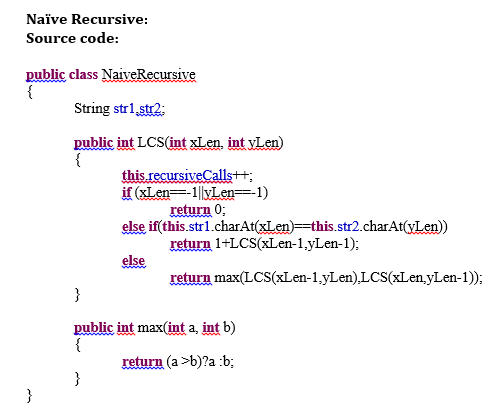
\includegraphics[width=2.5in]{f.jpg}
 	\caption{Source Code: Naive Recursive.}
 	
 	The source code for the Naive Recursive algorithm can be seen in the figure 1.
    
%	\item {Time Measuring Routines} \normalfont\newline
	Time Measuring Routines and Analysis:
	\end{normalsize}
		  	\end{figure}
		  	
	Naive Recursive calculates the LCS in Exponential time. The complexity is $O(2^n)$ in the worst case. The worst case happens when both the strings mismatch and their LCS is 0. The naïve recursive approach is not efficient in time as it computes the same sub-problem repeated number of times. The behavior of the Naive recursive is shown in the figures 2, 3, and 4 of this project.
	
    \begin{figure}[htb]
 	\begin{normalsize}
    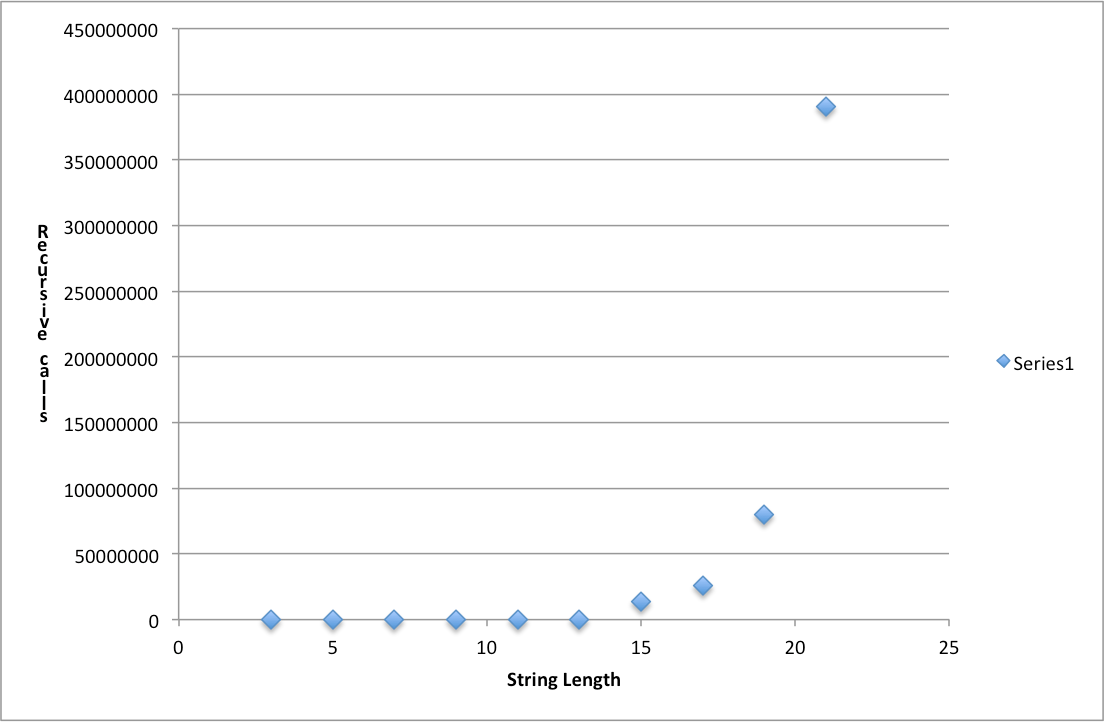
\includegraphics[width=2.5in]{n1.png}
    \caption{Recursive Calls vs String Length.}
	We can observe that the number of recursive calls increases exponentially as the input strings length increases.
	\end{normalsize}
	\end{figure}

	
	\begin{figure}[htb]
	\begin{normalsize}
	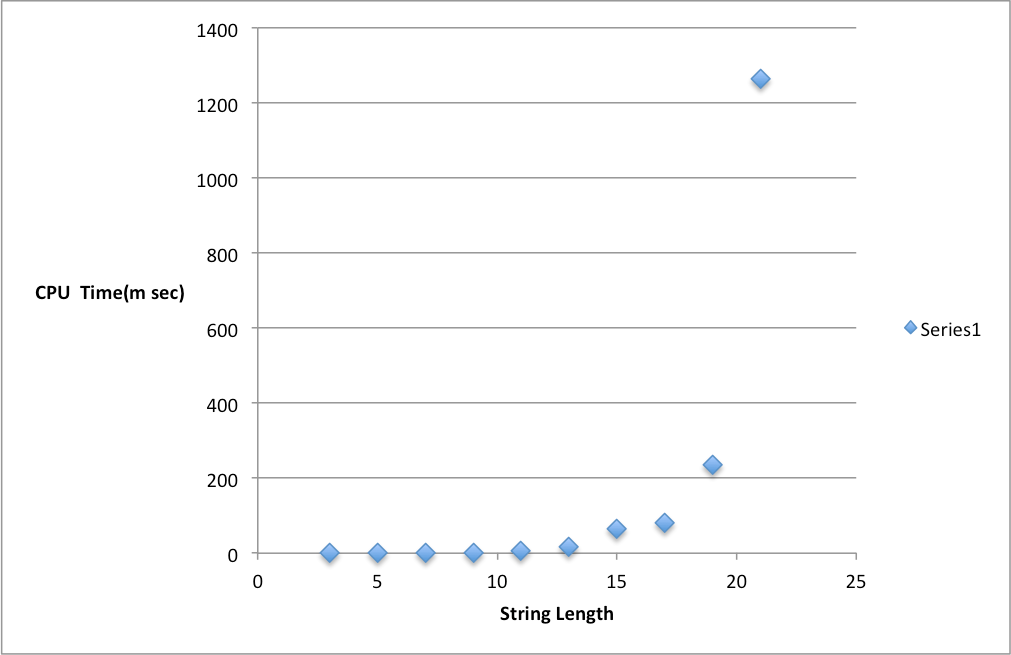
\includegraphics[width=2.5in]{n2.png}
  	\caption{CPU-Time vs String Length.}
  	
  	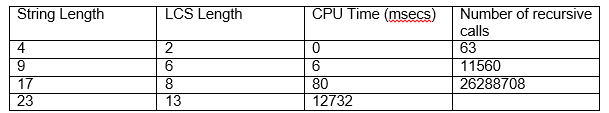
\includegraphics[width=2.5in]{n3.png}
  	\caption{Sample Output: Naive Recursive.}
  	
  	The Algorithm takes more than 10 sec when the input strings are of length around 20 and it runs for longer time even if the length is around 30.
  	 \end{normalsize}
  	 \end{figure}
  	 
  	 
  	 \begin{figure}[htb]
  	 \begin{normalsize}
  	The naive recursive is inefficient in terms of time taken but it is easier to implement and it doesn'\ t take extra space.
%}
%\end{enumerate}}

\subsection{Memoization Version}
%{\bf \begin{enumerate}
%\item {Source Code} {\normalfont\newline 
	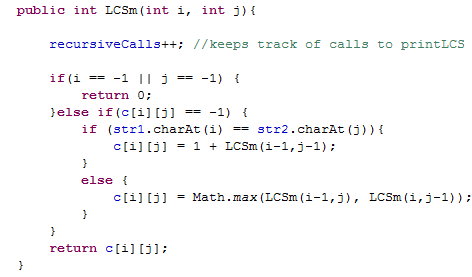
\includegraphics[width=2.5in]{m1.jpg}
  	\caption{Source Code1: Recursive Algorithm}
  	
	 The source code of the Memoization Algorithm version is shown in the figures 4 and 5 of this project.
	 \end{normalsize}
	 \end{figure}
	
	 
	\begin{figure}[htb]
	\begin{normalsize}
	 
  	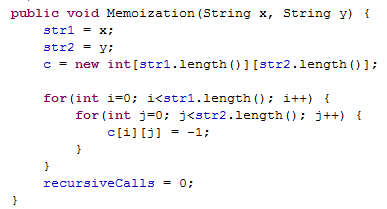
\includegraphics[width=2.5in]{m2.jpg}
  	\caption{Source Code2: Memoization}
  	
 	 The figure 5 is a method that belongs the source code of the Memoization Algorithm version.
 	\end{normalsize}
 	\end{figure}
 		
% }
%\item {Time Measuring Routines} {\normalfont

\begin{figure}[htb]
   \begin{normalsize}
   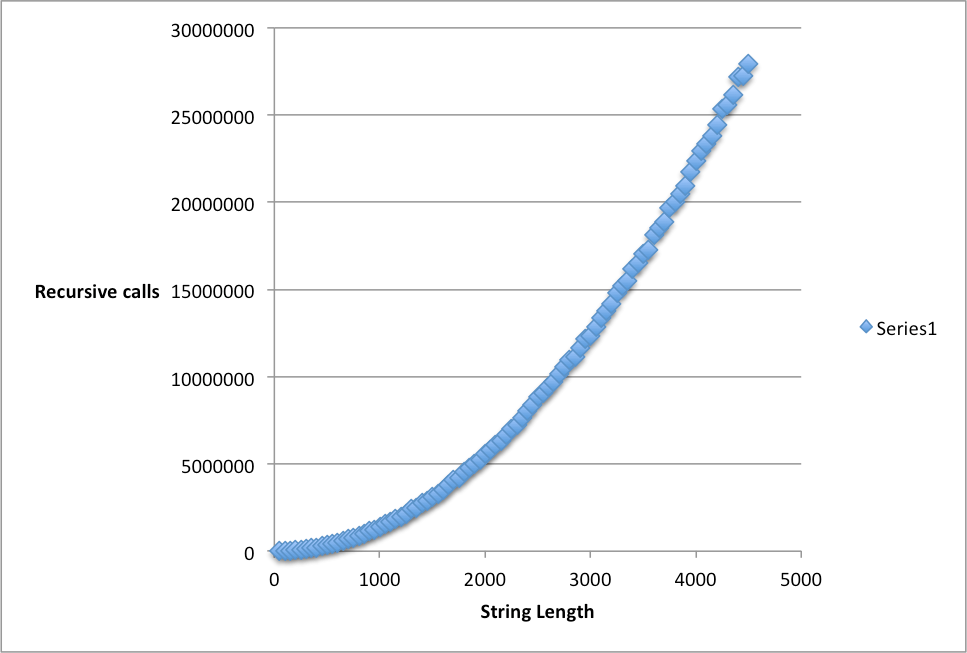
\includegraphics[width=2.5in]{m3.png}
   \caption{RecursiveCalls vs StringLength: Memoization}
   
   Memoization finds the longest common subsequence similar to Naive Recursive Algorithm but instead of a recursive call as in the case of naive recursive every time it computes the whether there is a entry in the table (Previous stored values). If its there it takes the result from these tables else it performs a recursive call and stored the result in the table.
   \end{normalsize}
    	\end{figure}
    
   
   \begin{figure}[htb]
   \begin{normalsize}
   
   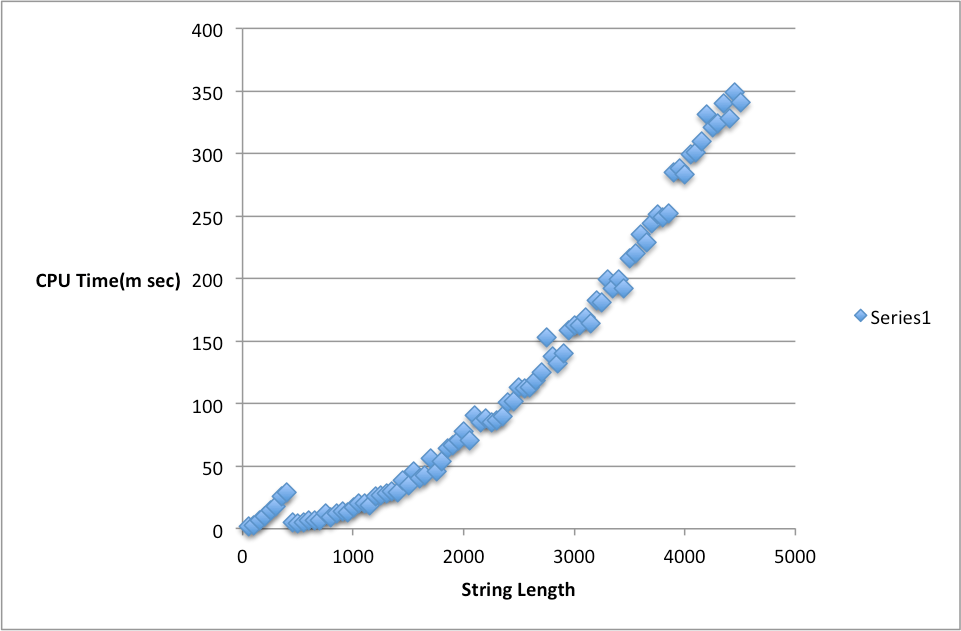
\includegraphics[width=2.5in]{m4.png}
   \caption{CPU TIME vs String Length: Memoization}
   
   The time complexity of Longest Common Subsequence is $O(n^3)$. As we are storing the intermediate results in a table which requires extra space. As the string size increases the table size increases (As in the Analysis below, when the string length is greater than 5690) and it run out of space throwing $"$Out of Memory Error: Java Heap Space$”$.
   \end{normalsize}
    	\end{figure}
    
    	
   \begin{figure}[htb]
   \begin{normalsize}
   
   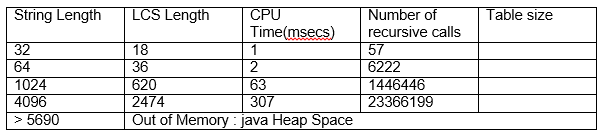
\includegraphics[width=2.5in]{m5.jpg}
   \caption{Output Sample: Memoization}
   
   The behavior of the algorithm is shown in the figures 7, 8 and 9.
   \newline
         
   Thus, Memoization is efficient when the strings are of smaller length and is not good to use when the strings are of larger length because of memory usage (As discussed above) and cubical time growing.
   
   \end{normalsize}
   \end{figure}
  
       
   \begin{figure}[htb]
   \begin{normalsize}
   Its not possible to reach scenario where the algorithm takes more than 10 secs since It runs out of space.

%}
%\end{enumerate}}

\subsection{Dynamic programming Version}
%{\bf \begin{enumerate}
%\item {Source Code} {\normalfont 
 \
  	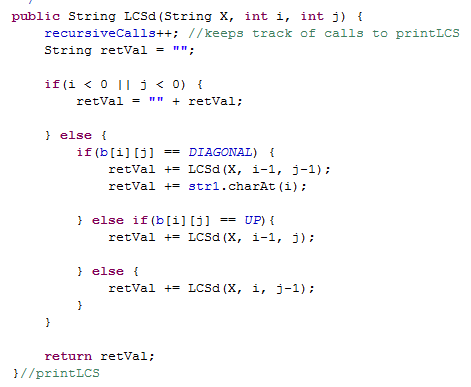
\includegraphics[width=2.5in]{d1.jpg}
  	\caption{Source Code1: Dynamic Algorithm}
  	
 	 The figure 10 is the source code for the Dynamic Algorithm, and the figure 11 is a method that belongs to the source code of the Dynamic Algorithm.
 	 
 	 \end{normalsize}
 	 \end{figure}
 	 
 	  
 	  
 	 \begin{figure}[htb]
 	 \begin{normalsize}
     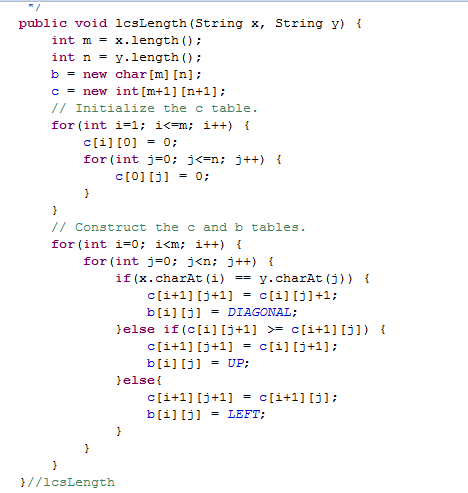
\includegraphics[width=2.5in]{d2.jpg}
     \caption{Source Code2: Dynamic Algorithm}
     
     \end{normalsize}
     \end{figure}
      
 	
%}

%\item {Time Measuring Routines} {\normalfont\newline 
 \begin{figure}[htb]
 \begin{normalsize}
   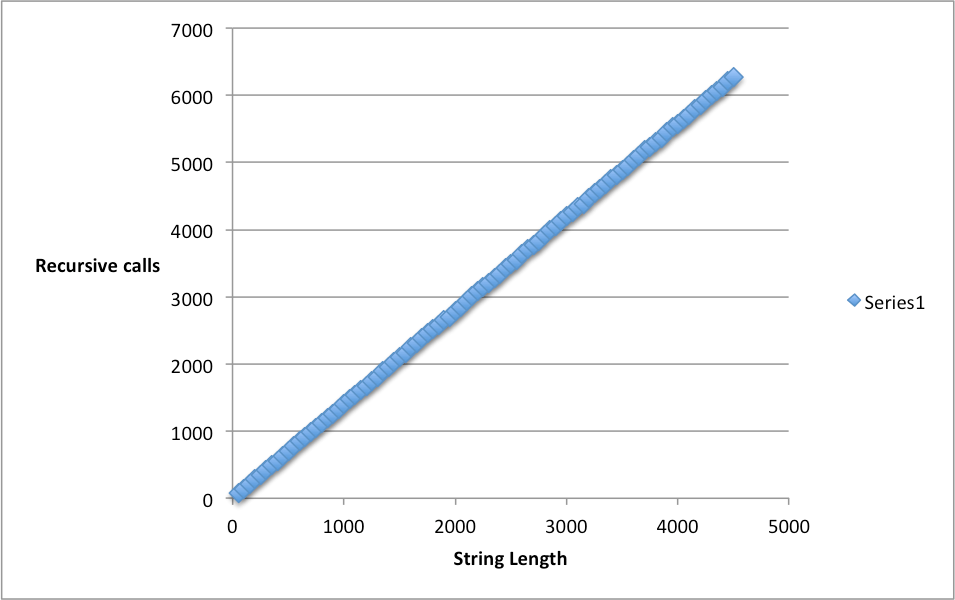
\includegraphics[width=2.5in]{d3.png}
   \caption{Recursive Calls vs String: Dynamic Programming}
   
  	As Contrary to Memoization, Dynamic Programming follows the  $“$Bottom up approach$”$. It solves the sub problems first, filling up an n-dimensional table. Based on the results in the table , the solution to the $“$top$”$ original problem is then computed. The time complexity of the LCS using Dynamic Programming is O(mn), where m and n are the length of the input strings. Thus Dynamic programming solves the LCS in Quadratic time but it also takes quadratic space. The performance of the Dynamic Programming algorithm can be observed in the figures 12, 13, and 14 in this project.
    
    \end{normalsize}
  	\end{figure}
    
    
   	\begin{figure}[htb]
   	\begin{normalsize}
    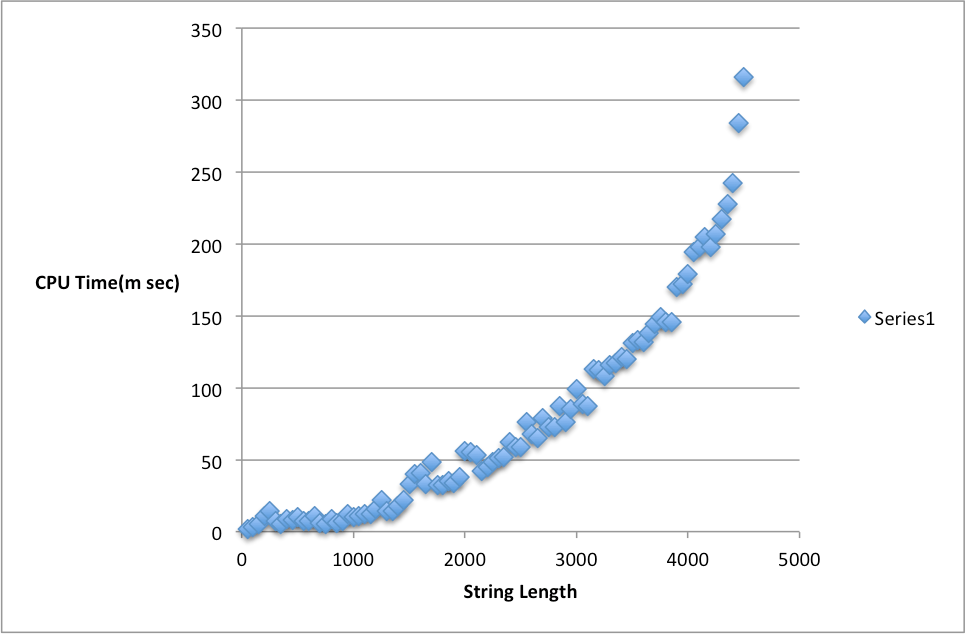
\includegraphics[width=2.5in]{d4.png}
    \caption{CPU Time vs String Length: Dynamic Programming}
    
   	As it also takes Quadratic space, It suffers from the limitation which we have faced for Memoization. It cannot take handle strings of length greater than 5690 as the program runs out of memory throwing exception $“$Out of Memory Error: Java Heap Space$”$. But it is efficient as compared to Memoization as it runs it quadratic time contrary to Memoization, which takes cubic time. 
   
   	\end{normalsize}
   	\end{figure}
   	

    \begin{figure}[htb]
   	\begin{normalsize}
    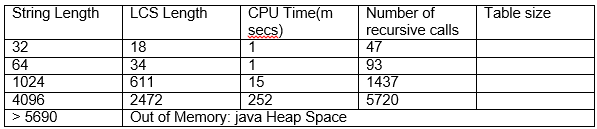
\includegraphics[width=2.5in]{d5.jpg}
    \caption{Sample Output: }
    
    Its not possible to reach scenario where the algorithm takes more than 10 sec since It runs out of space similar to Memoization.
    
\end{normalsize}
\end{figure}


%}
%\end{enumerate}}

\subsection{Quadratic-time linear-space Version}
%{\bf \begin{enumerate}
%\item {Source Code} {\normalfont\newline 
\begin{figure}[htb]
\begin{normalsize}
 	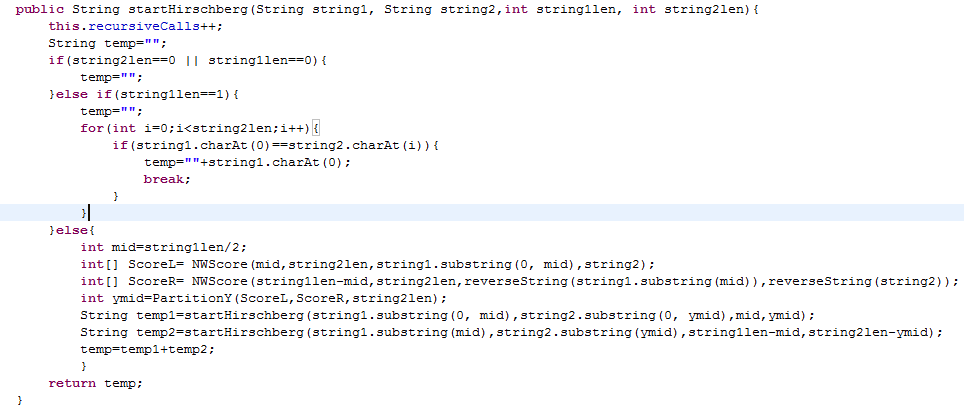
\includegraphics[width=2.5in]{h1.jpg}
 	\caption{Source Code1: Hirschberg.}
 	
  	The source code for the Hirschberg algorithm is shown in the figure 15. Also, you can see two main methods that belong to the Hirschberg algorithm. These methods are shown in figures 16 and 17.
  	
  	\end{normalsize}
  	\end{figure}
  	
  	
  	 
  	 \begin{figure}[htb]
  	 \begin{normalsize}
   	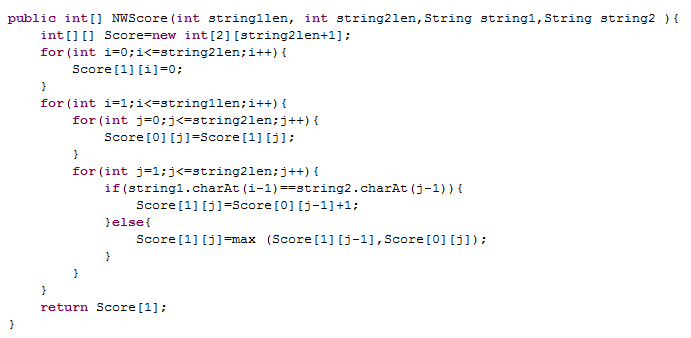
\includegraphics[width=2.5in]{h2.jpg}
   	\caption{Source Code2: Hirschberg.}
   	
    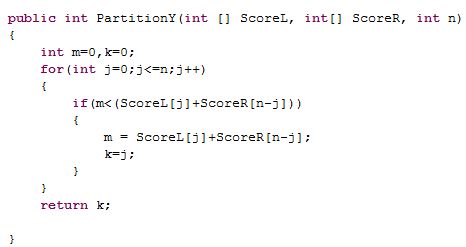
\includegraphics[width=2.5in]{h3.jpg}
    \caption{Source Code3: Hirschberg.}
    
    \end{normalsize}
    \end{figure}
      	

%}

%\item {Time Measuring Routines} {\normalfont\newline
\begin{figure}[htb]
\begin{normalsize}
	Hirschberg finds the longest Common subsequence by recursively dividing the problem into sub-problem, It finds the LCS in a quadratic time and in linear space, An improvement over Dynamic Programming Algorithm which takes quadratic time and quadratic space. The algorithm takes o(p(m+1-p)logn) where p is the length of the Longest common subsequence. m and n are lengths of the Input strings such that m<= n. 
	\newline
	The behavior of the algorithm is shown in the figures 18,19, and 20 in this project.
	
 	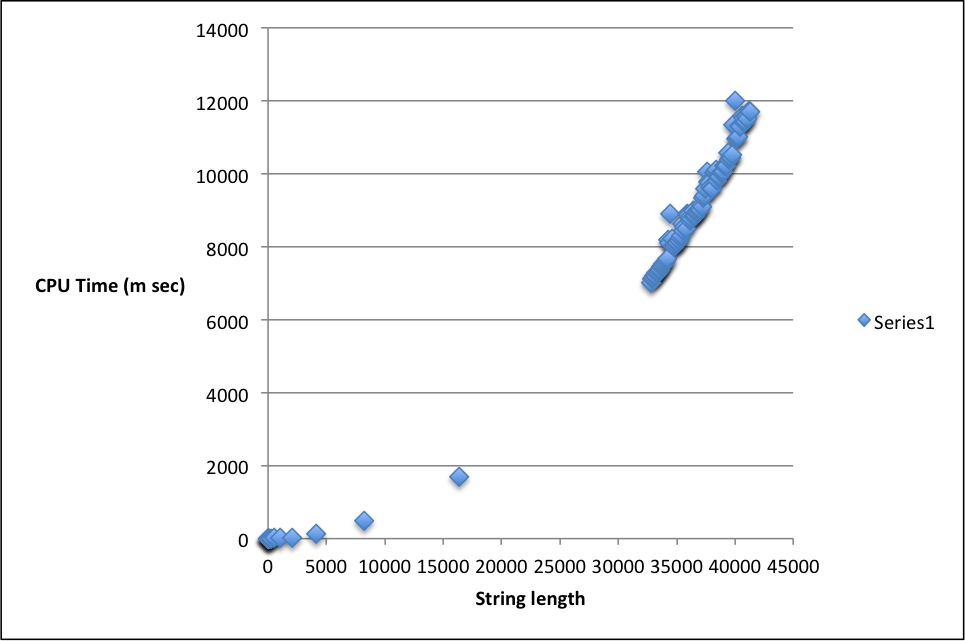
\includegraphics[width=2.5in]{71.png}
  	\caption{CPU-Time vs String Length: Hirschberg.}
  	 \end{normalsize}
  	 \end{figure}
  	
    \begin{figure}[htb]
  	\begin{normalsize}
	The Algorithm takes more than 10 sec when the input strings are of length around 20 and it runs for longer time even if the length is around 30.
	
 	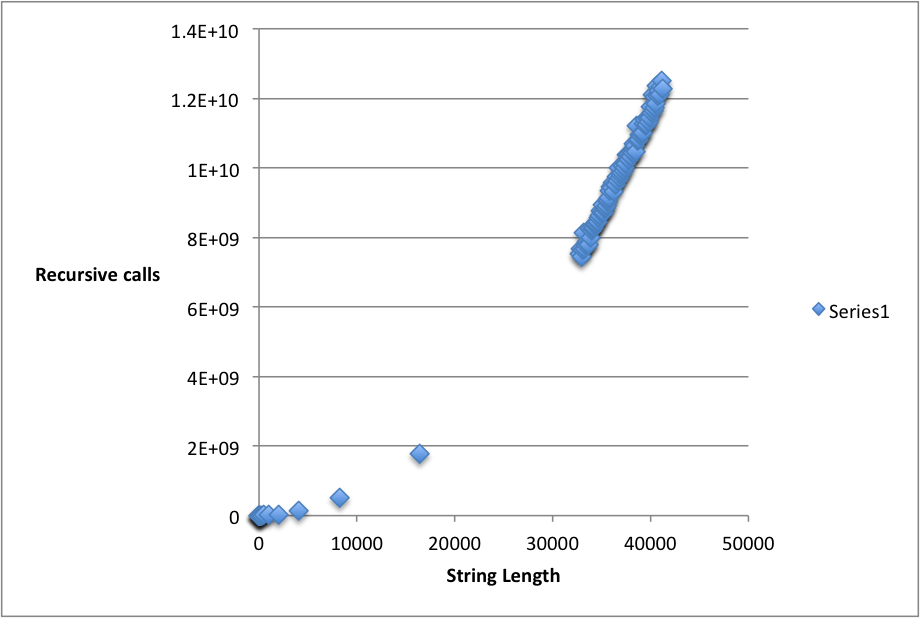
\includegraphics[width=2.5in]{72.png}
 	\caption{Recursive Calls vs String Length: Hirschberg.}
 	
 	\end{normalsize}
 	\end{figure}\clearpage
 	  	 
 	
 	\begin{figure}[htb]
 	\begin{normalsize}
	We can observe that the number of recursive calls increases exponentially as the input strings length increases.
	
    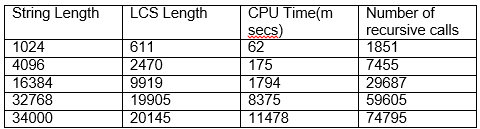
\includegraphics[width=2.5in]{h6.jpg}
    \caption{Sample Output: Hirschberg.}
    
    The Algorithm takes more than 10 sec when the Input size is approximately greater than the 34000. The Algorithm is efficient as it can process longer string in very less time than as compared to other algorithms discussed above in the previous sections. 
    \newline
    The naive recursive is inefficient in terms of time taken but it is easier to implement and it doesn'\ t take extra space.
    
 \end{normalsize}
 \end{figure}
 
%}
%\item {Sample Profile Run} {\normalfont\newline
\begin{figure}[htb]
\begin{normalsize}
   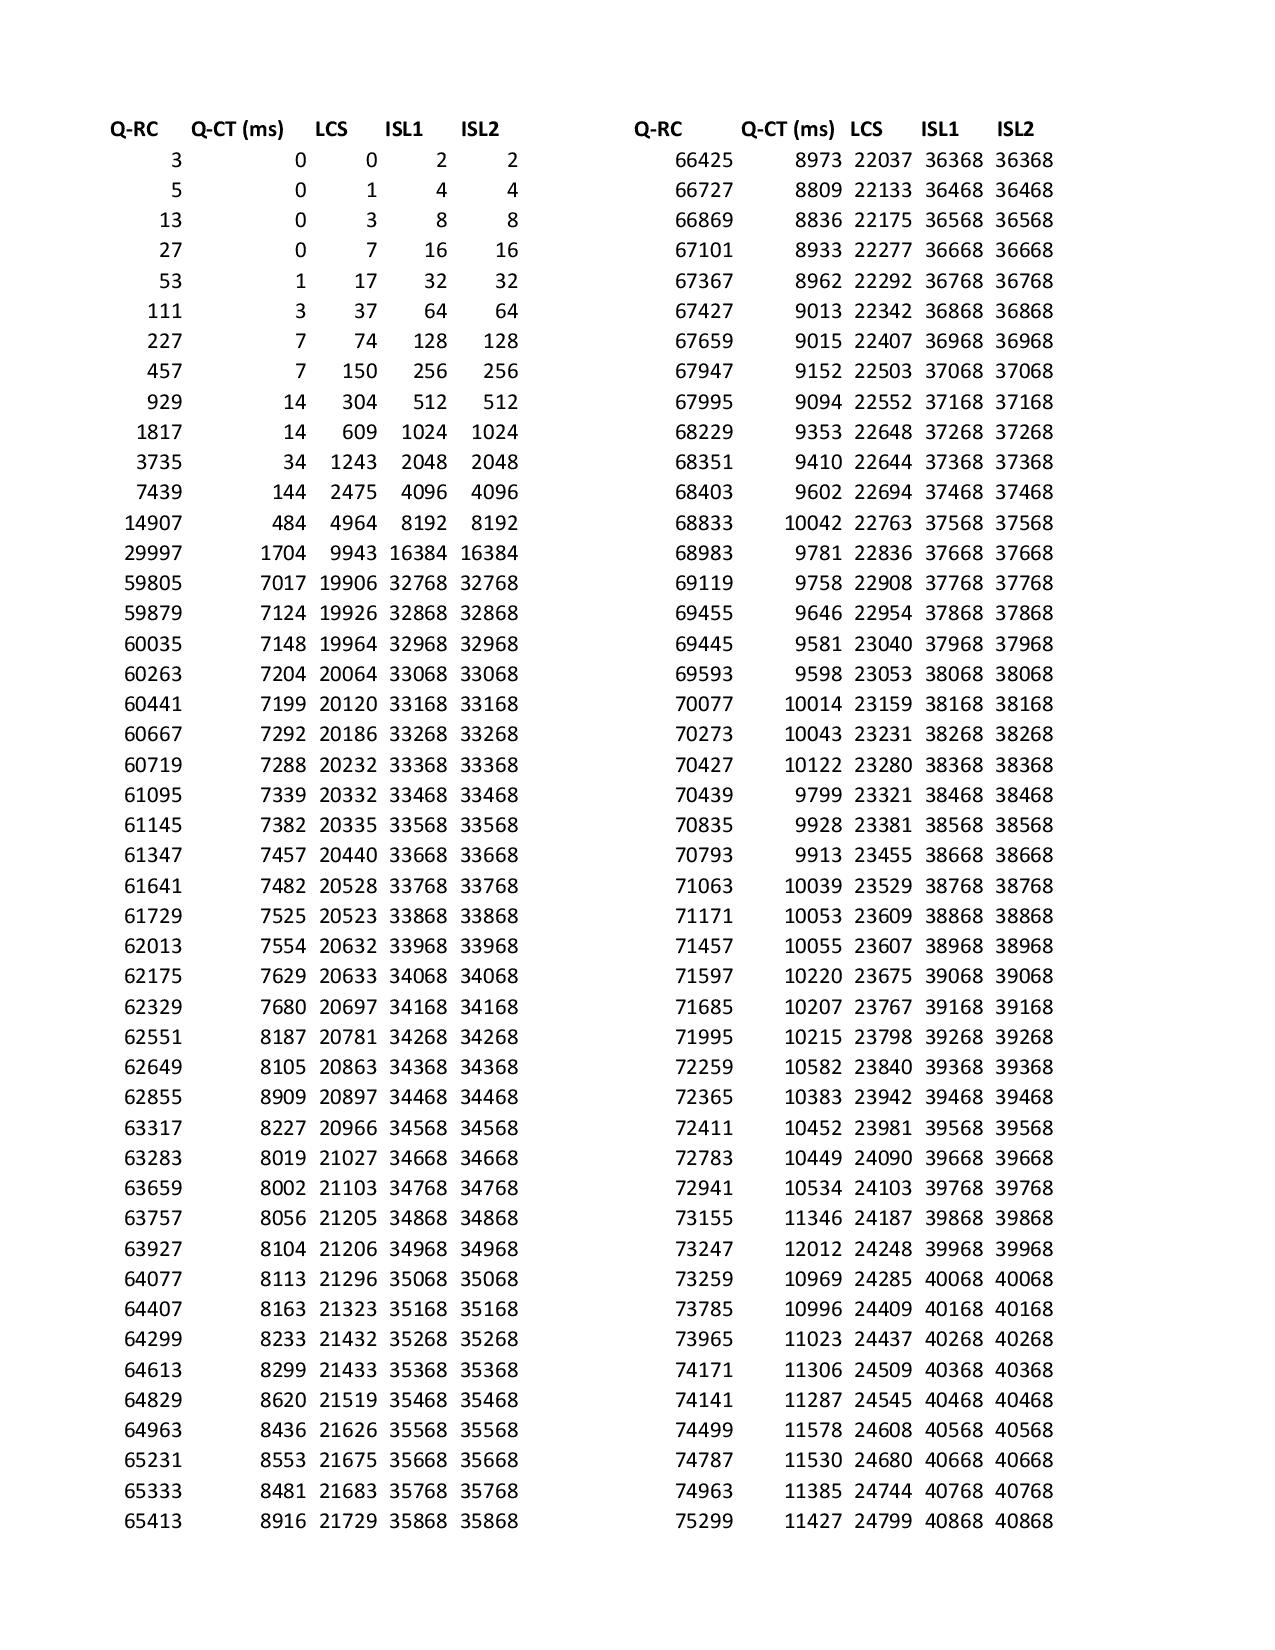
\includegraphics[width=2.5in]{hspr-1.jpg}
   \caption{Sample Profile Run: Hirschberg.}
   
 	The sample profile run can be seen in the figure 21 and 22. 
 	
   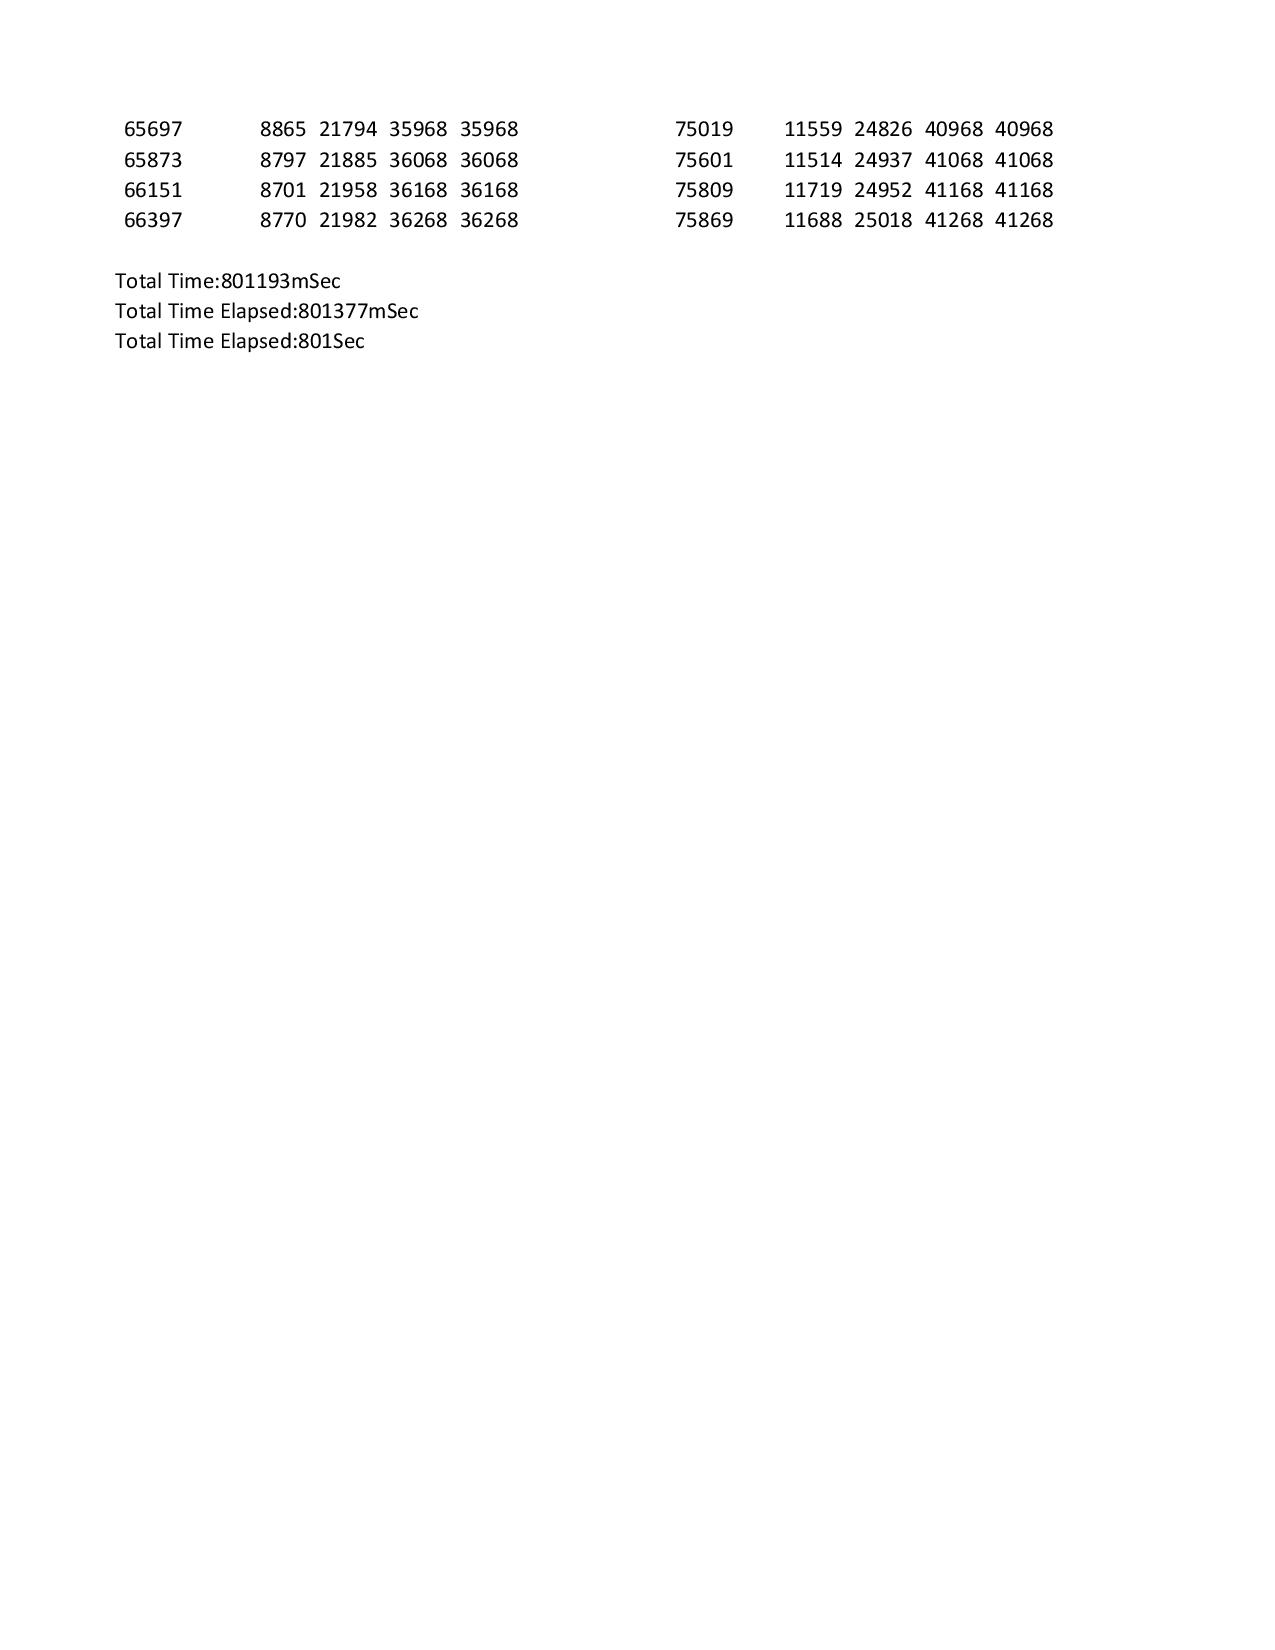
\includegraphics[width=2.5in]{hspr-2.jpg}
   \caption{Sample Profile Run: Hirschberg.}
   
\end{normalsize}
\end{figure}

%}
%\end{enumerate}}

%\section{Comparison}
\label{mistakes}
%{\bf \begin{enumerate}
%\item {a } {\normalfont\newline 
\begin{figure}[htb]
\begin{normalsize}
Analyzing the behavior of all the four algorithms discussed above using the  same Input cases. We get the results shown in the figures 23, 24, 25 and 26. 

    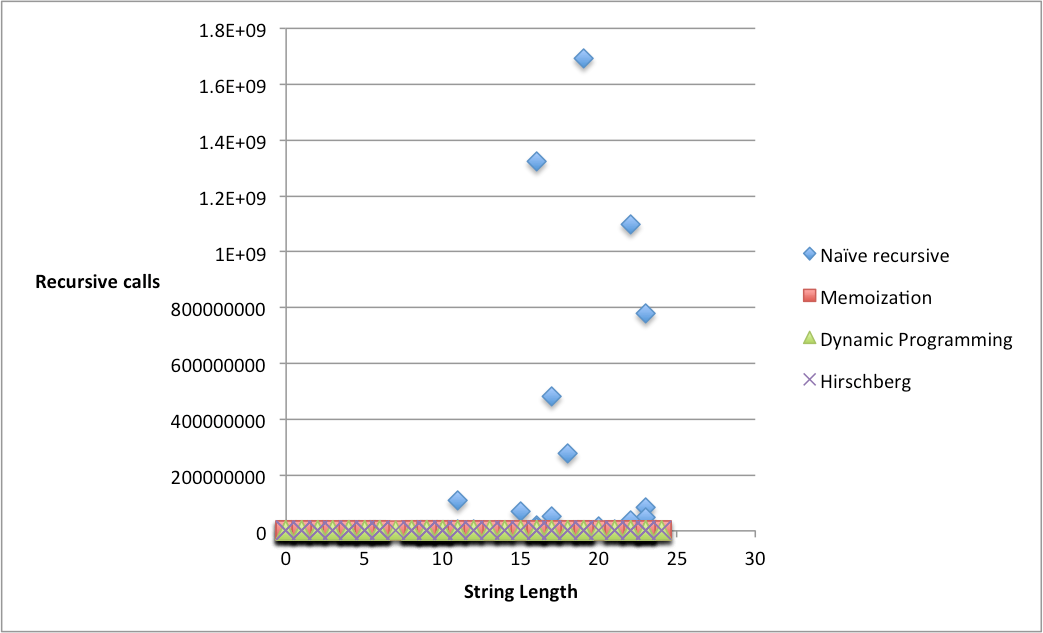
\includegraphics[width=2.5in]{c1.png}
    \caption{Recursive Calls vs String Length: All Algorithms}
    
	As we can observe, the number of recursive calls for algorithms other than naive recursive is negligible than compared to naive recursive algorithm since the naive recursive take exponential time to find the LCS.
	
	\end{normalsize}
	\end{figure} 
	
	\begin{figure}[htb]
	\begin{normalsize}
    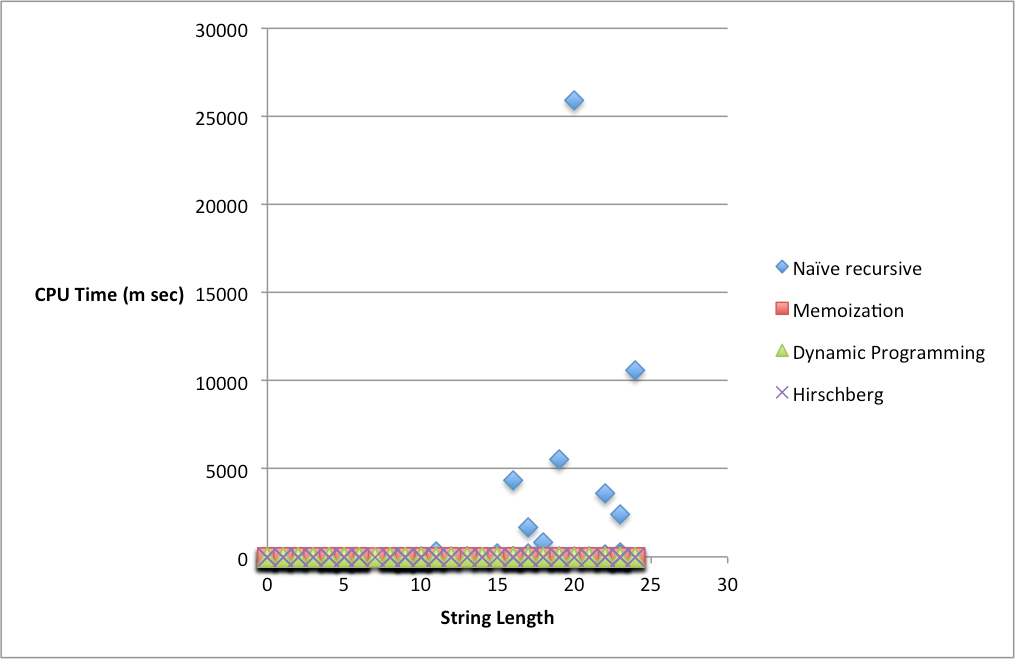
\includegraphics[width=2.5in]{c2.png}
    \caption{CPU TIME vs String Length: All Algorithms}
    
    Same as for recursive calls, the CPU time for algorithms other than naive recursive is negligible than compared to naive recursive algorithm since the naive recursive take exponential time to find the LCS.
    \end{normalsize}
    \end{figure} 
    
    
    \begin{figure}[htb]
    \begin{normalsize}
    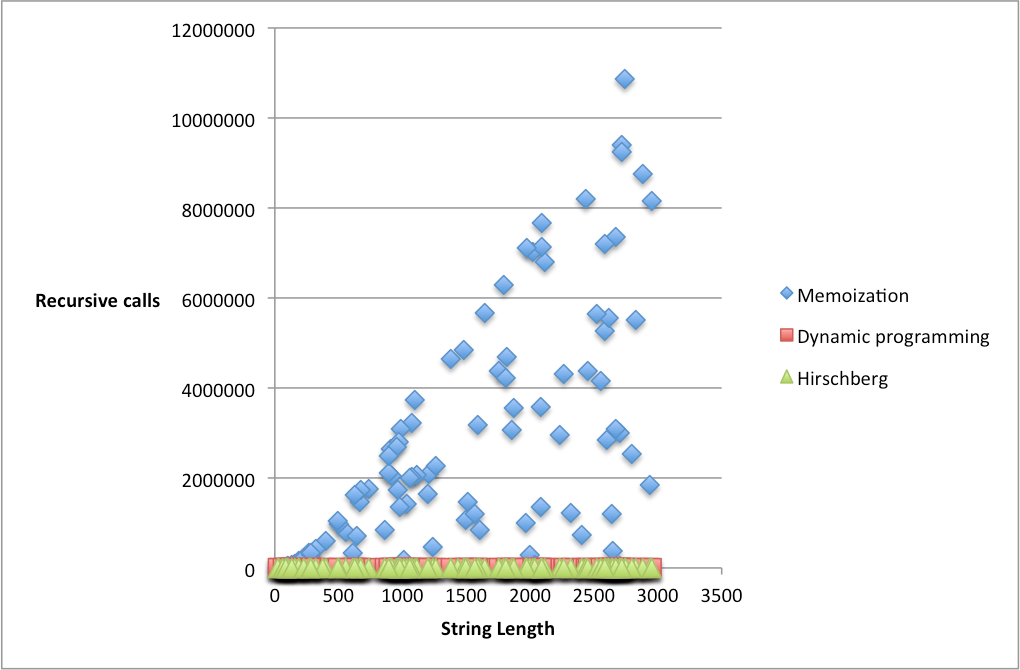
\includegraphics[width=2.5in]{c3.png}
    \caption{CPU TIME vs String Length: All Algorithms Except Naive Recursive]}
    
    We have excluded the naive recursive approach to get an effective comparison of the Memoization, Dynamic Programming and Hirschberg algorithms. We can observe that the Memoization has more number of recursive calls than the Dynamic Programming and Hirschberg, which has cubic time complexity as compared to the Hirschberg and Dynamic Programming algorithms. It also indicates that the dynamic programming and Hirschberg algorithms have similar number of recursive calls for same input string.
    
    \end{normalsize}
    \end{figure} 
        	
       
    \begin{figure}[htb]
    \begin{normalsize} 	
    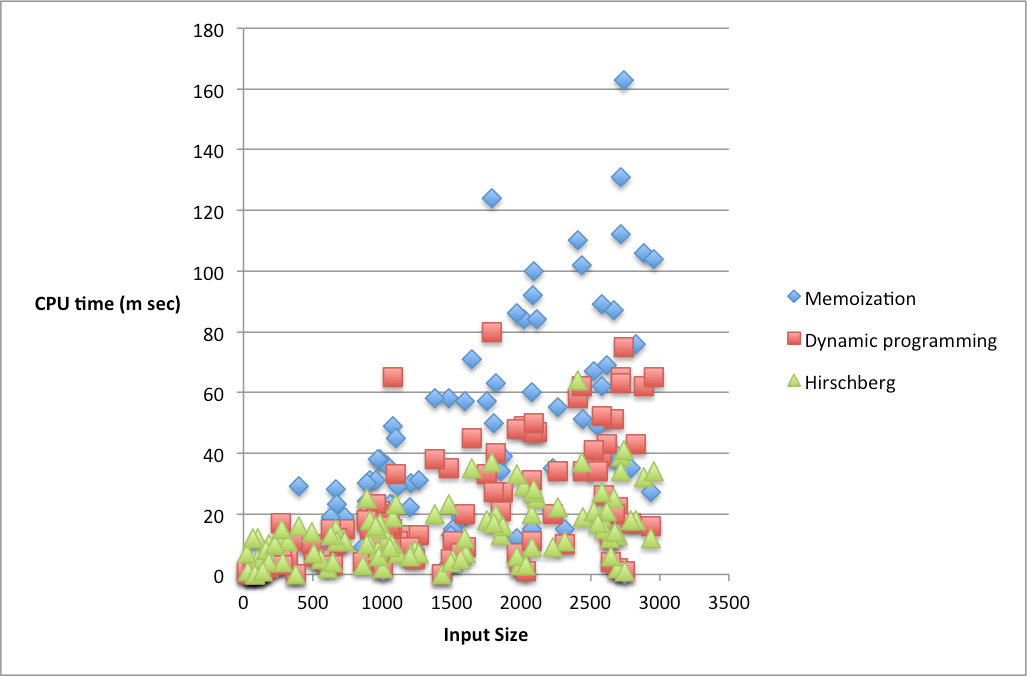
\includegraphics[width=2.5in]{c4.png}
    \caption{CPU TIME vs InputSize: For all algorithms except Naive Recursive algorithms.}
    
    Though, the Hirschberg and Dynamic Programming has similar number of recursive calls but Hirschberg outperforms the dynamic programming comparatively in CPU time taken to process the same Input random Strings. The figure of these measurements can be seen in the figure 26.
     
\end{normalsize}
\end{figure}    

%}
%\end{enumerate}}

\section{Algorithms High Level Script}
\begin{figure}[htb]
\begin{normalsize}
     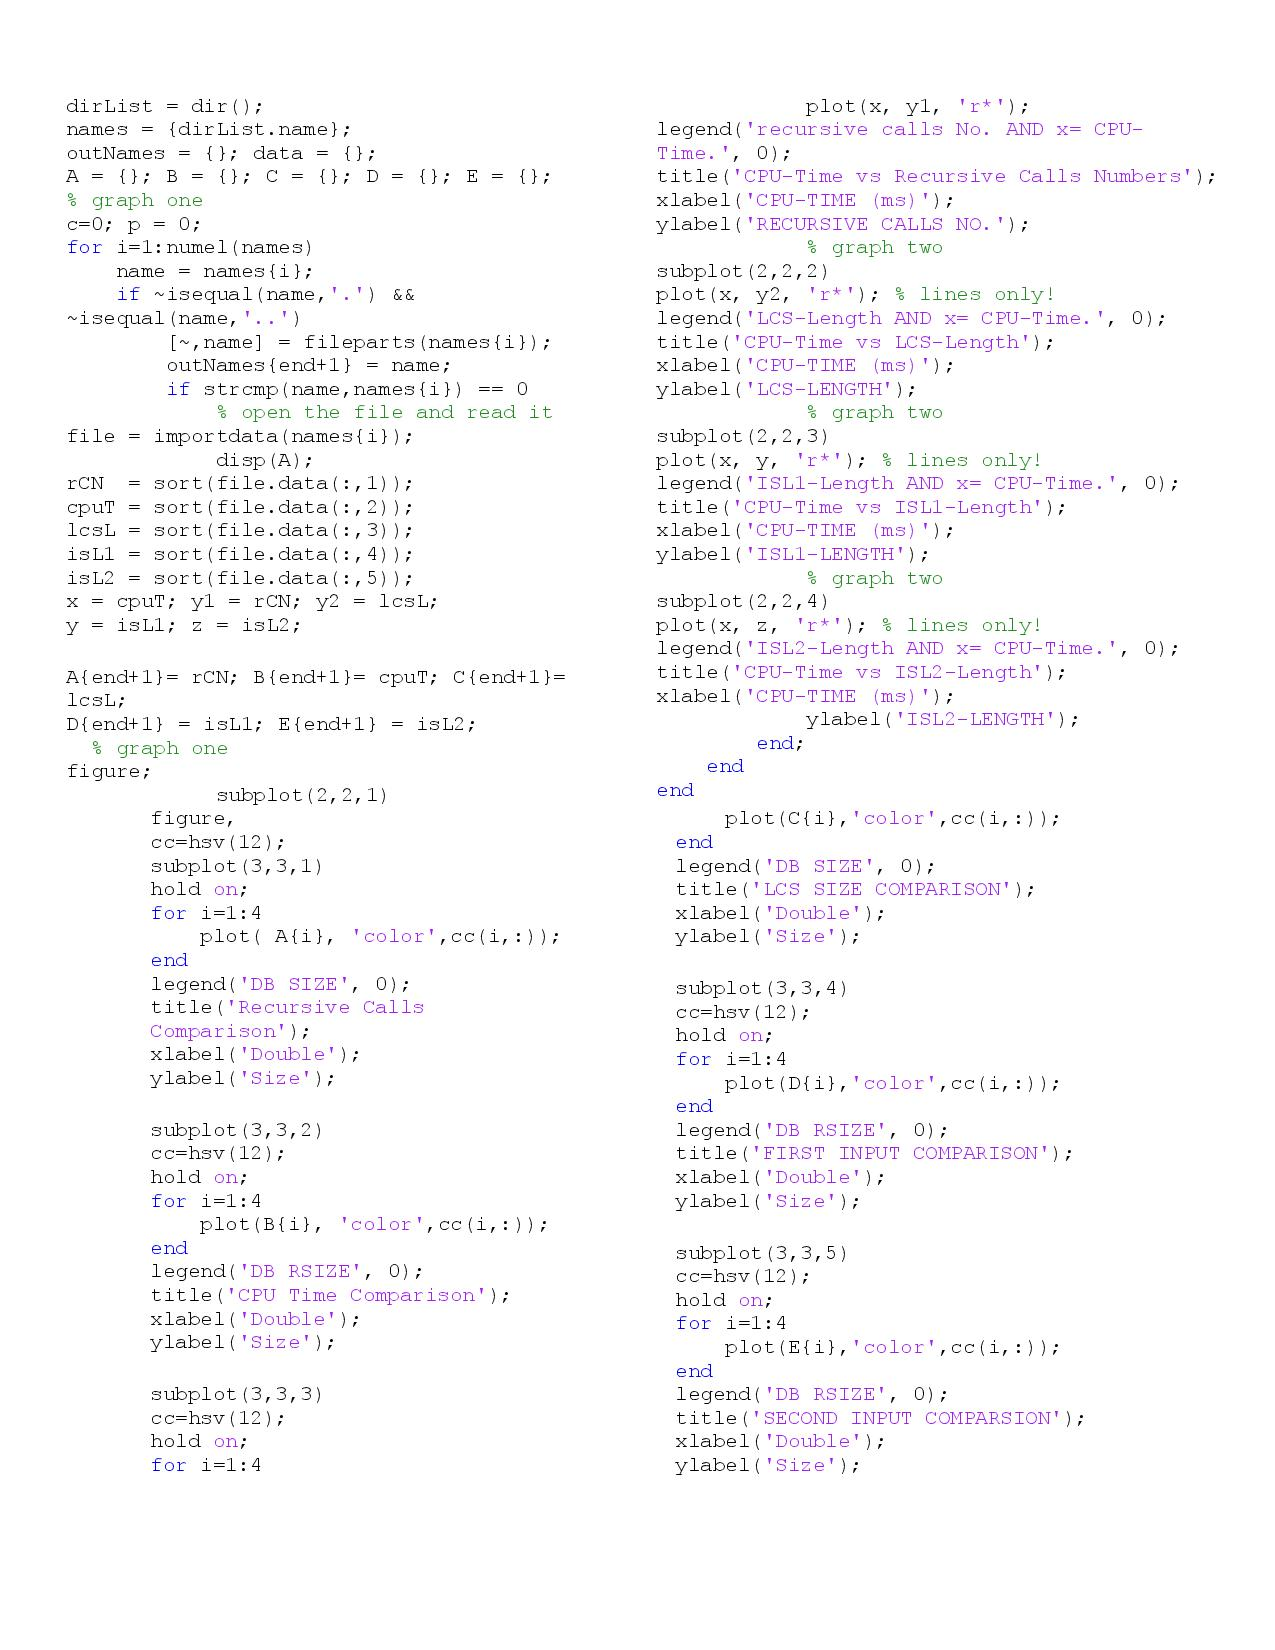
\includegraphics[width=3.8in]{./HLSm}
     \caption{Matlab - High Level Script: To Test All Algorithm}
     
     The code in the figure 27 is the high level script we use to analyze the performance and behavior of each one of the algorithm already tested and individually analyzed above. This script takes the time sequence, number of recursive calls, and LCS length along with its inputs lengths recorder by other high level scripts and graphs their performance for comparison purpose. In fact, this high level script takes the components mentioned above of each algorithm and graph them separately for a better understanding of these algorithm performance. 
         
     \end{normalsize}
     \end{figure}
      
         
     \begin{figure}[htb]
     \begin{normalsize}
     \includegraphics[width=3.0in]{./HLS1}
     \caption{Matlab - High Level Script: To Test Dynamic Programming}
     
     The performance of the dynamic programing algorithm is shown in the figure 28. 
     
     \end{normalsize}
     \end{figure}
     
     \begin{figure}[htb]
     \begin{normalsize}
     \includegraphics[width=3.0in]{./HLS2}
     \caption{Matlab - High Level Script: To Test Memoization}
	 Also, the figure for the Memoization version of the recursive algorithm can be seen in the figure 29.
    
    \end{normalsize}
    \end{figure}
    
    \begin{figure}[htb]
    \begin{normalsize}              
     \includegraphics[width=3.0in]{./HLS3}
     \caption{Matlab - High Level Script: To Test Naive Recursive Algorithm}
     
     The performance of Naive Recursive algorithm can be seen in figure 30.
     
     \end{normalsize}
     \end{figure}
     
     \begin{figure}[htb]
     \begin{normalsize}                  
     \includegraphics[width=3.0in]{./HLS4}
     \caption{Matlab - High Level Script: To Test Hirschberg Algorithm}
     Similarly, we can see the performance of the Hirschberg algorithm in the figure 31. 
 
     \end{normalsize}
     \end{figure}
            
   
     \begin{figure}[htb]
     \begin{normalsize}                
     \includegraphics[width=3.0in]{./HLS}
     \caption{Matlab - High Level Script: To Test All Algorithm}
	 In Matlab, we also were able to measure and compare the overall performance of all algorithms. This last test was performed by section, each graph represent a different section that contribute to the algorithm performance. These sections are the number of recursive calls, the cpu time, tne LCS length and the length of the input strings. 
	 
\end{normalsize}
\end{figure}

     \begin{figure}[htb]
     \begin{normalsize}                
     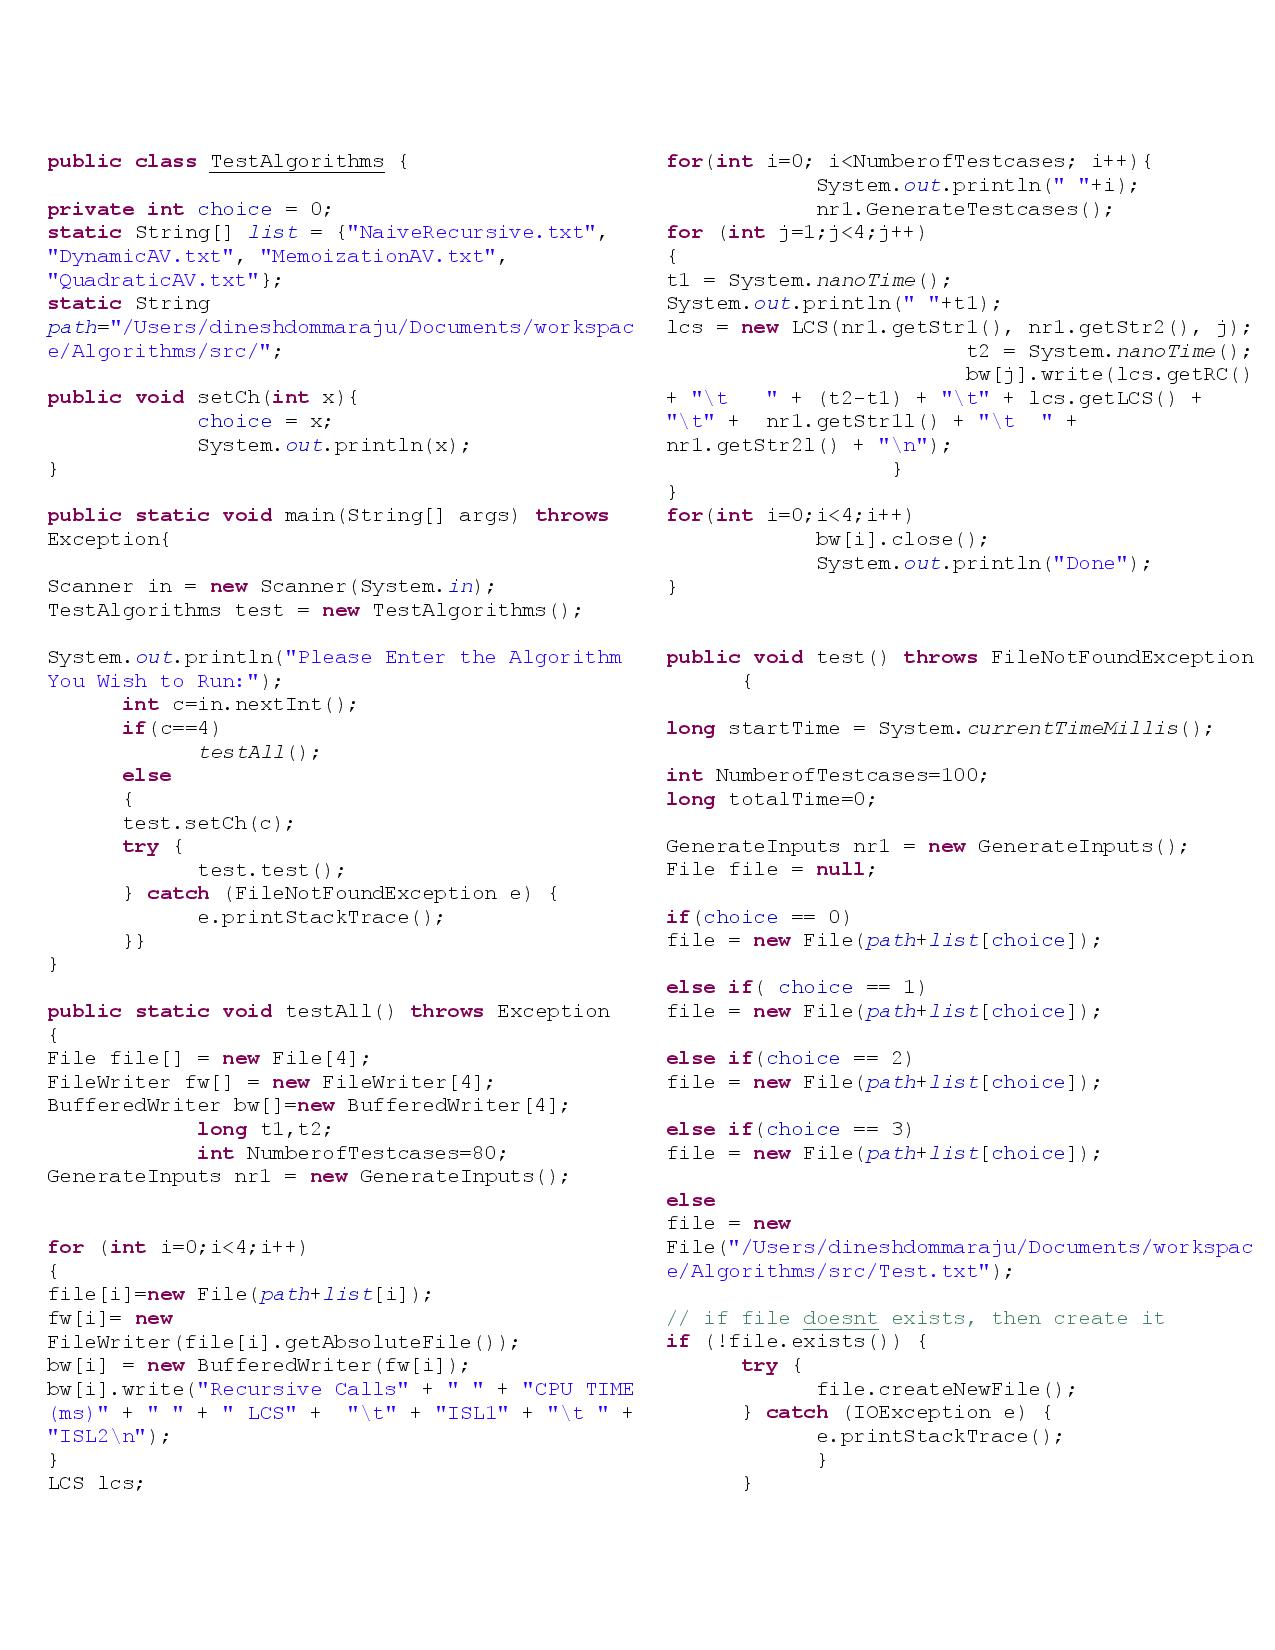
\includegraphics[width=3.0in]{./TestData1}
     \caption{Java Code - High Level Script: To Test All Algorithm}
     
     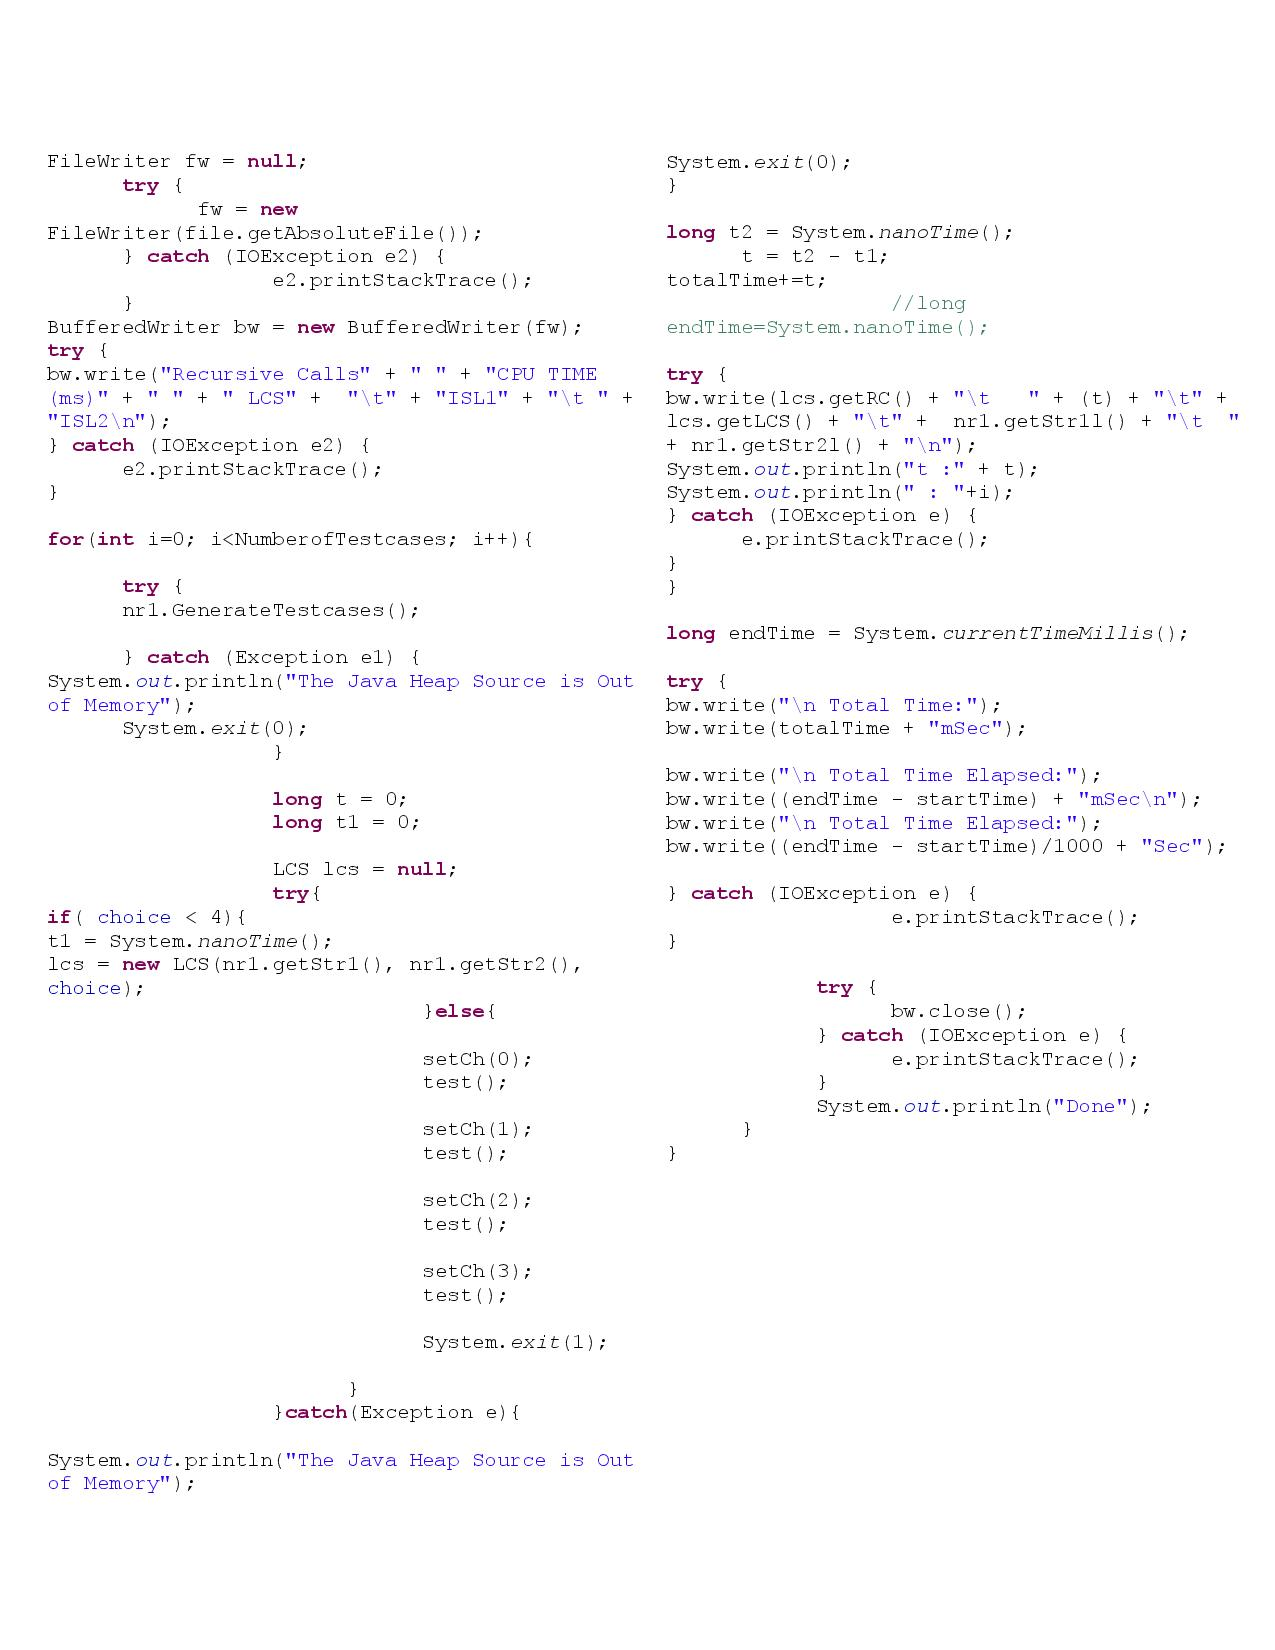
\includegraphics[width=3.0in]{./TestData2}
          \caption{Java Code - High Level Script: To Test All Algorithm}
          
	The figures 33 and 34 are the images of the source code we used to record the data of the time and recursive calls done by each one of the algorithm along with the length of its inputs and LCS. This code recored the time takes the time that each algorithm takes to generate the LCS from the two input strings. These data along with the number of recursive calls and length of the input and LCS string is recorded on a text file. These text files is later access by our Matlab and Excel High Level Script to simulate each algorithm performance.
	 
\end{normalsize}
\end{figure}



\section{Sample Profiles Run}    
 %{\bf \begin{enumerate}
 %\item {Sample Profile I} {\normalfont\newline 
 \begin{figure}[htb]
 \begin{normalsize}
      The three images in figure 35, 36  and 37 are a demonstration of the profile run of each one of the algorithms in nanoseconds.
      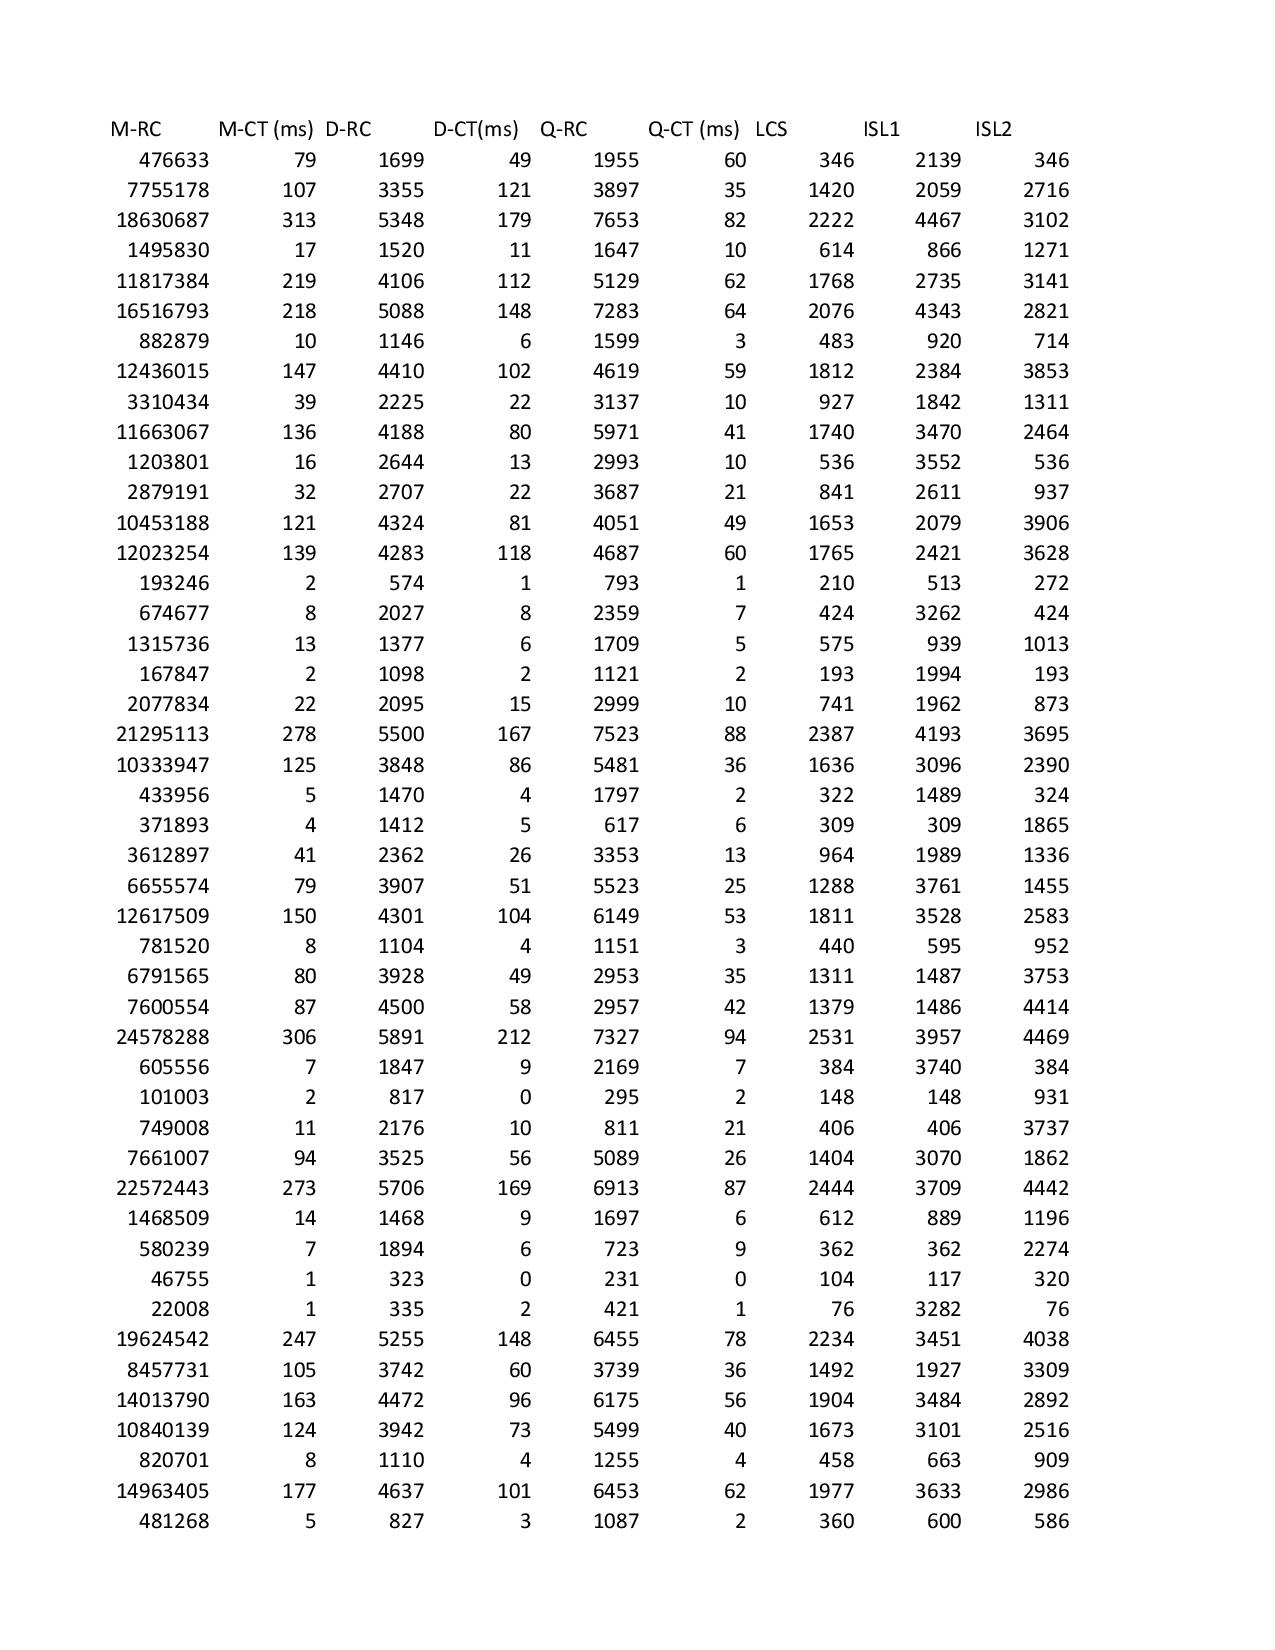
\includegraphics[width=2.5in]{52(1).jpg}
      \caption{Sample Profile Run1 in Nanoseconds}
      
      \end{normalsize}
      \end{figure}
      
      \begin{figure}[htb]
      \begin{normalsize}
      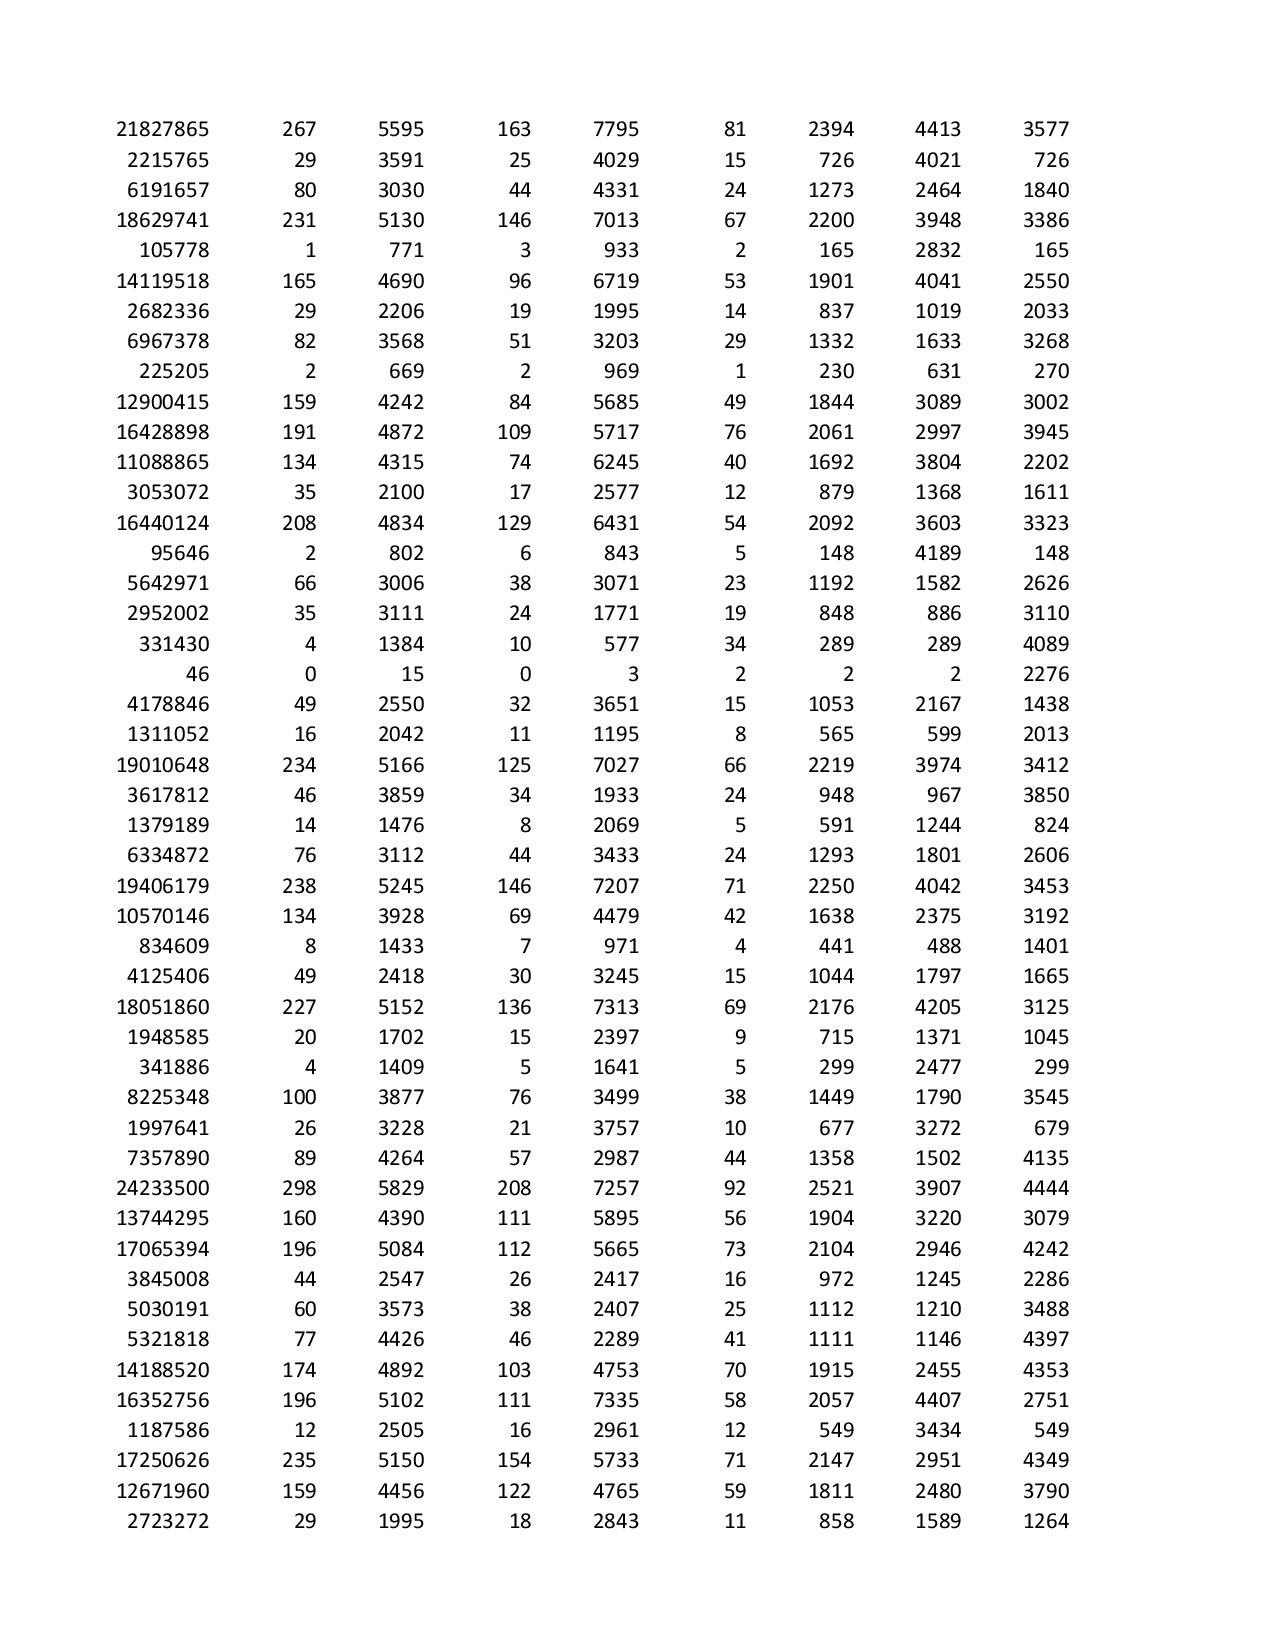
\includegraphics[width=2.5in]{52(2).jpg}
      \caption{Sample Profile Run2 in nanoseconds.}
  
      \end{normalsize}
      \end{figure}
        
      \begin{figure}[htb]
      \begin{normalsize}
      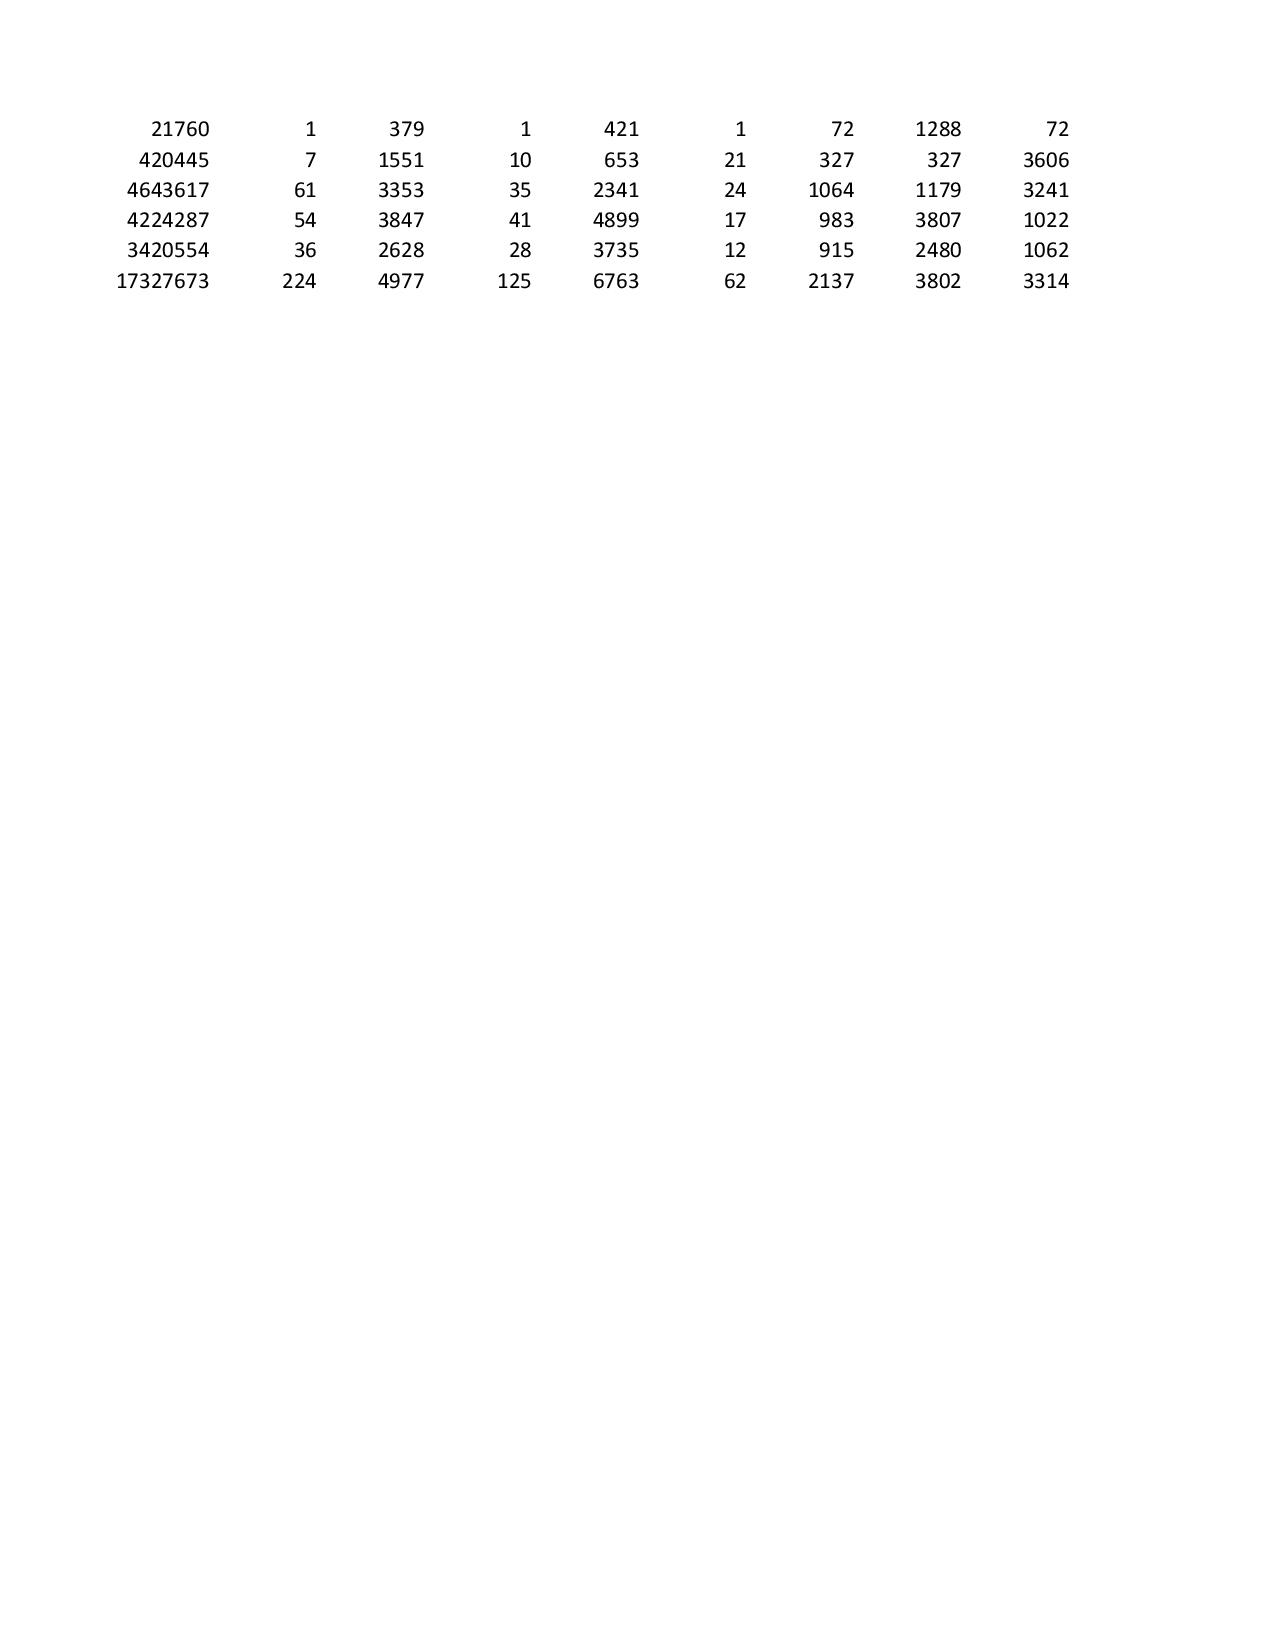
\includegraphics[width=2.5in]{52(3).jpg}
      \caption{Sample Profile Run3 in nanoseconds.}
      
      \end{normalsize}
      \end{figure}
      
      \begin{figure}[htb]
      \begin{normalsize}         
      The three images in figure 38, 39  and 40 are a demonstration of the profile run of each one of the algorithms in microseconds. 
        
      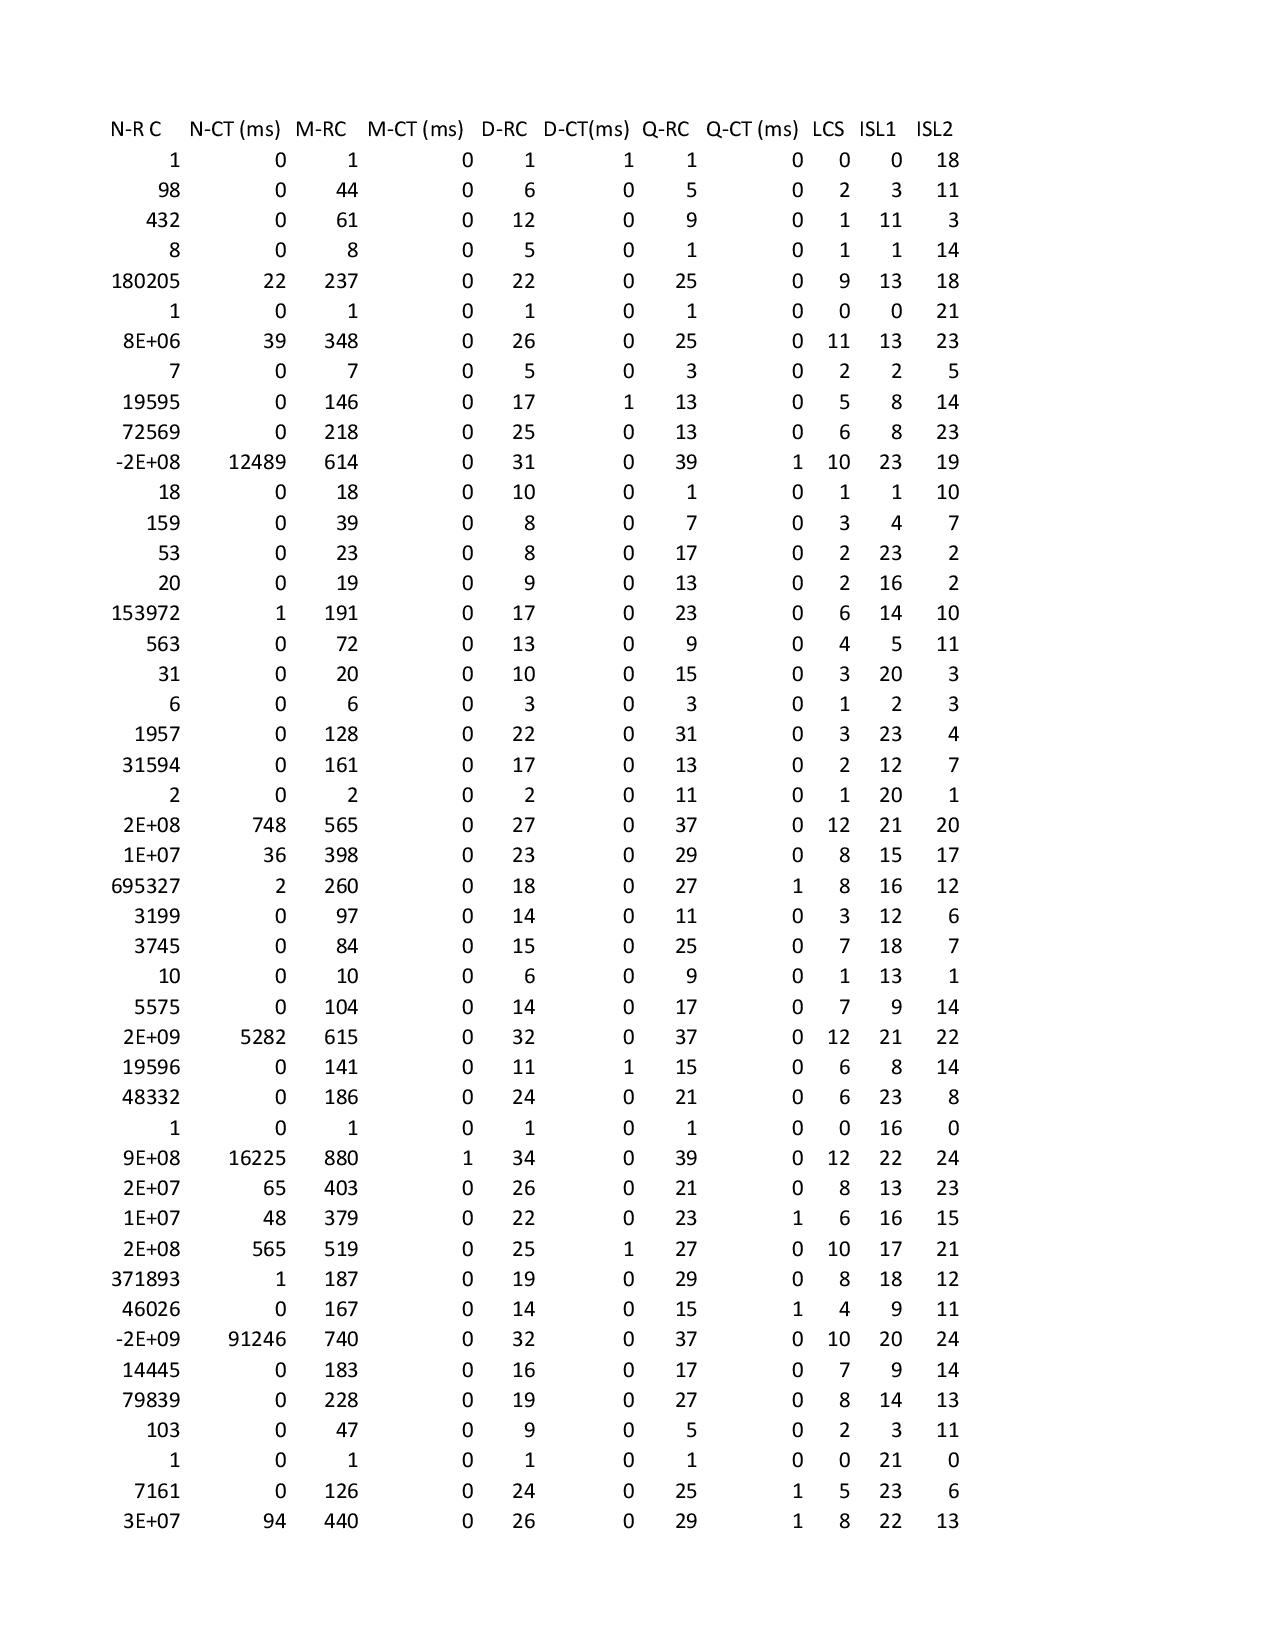
\includegraphics[width=2.5in]{51(1).jpg}
      \caption{Sample Profile Run1 in milliseconds.}
        
      \end{normalsize}
      \end{figure}
                            
      \begin{figure}[htb]
      \begin{normalsize} 
                            
      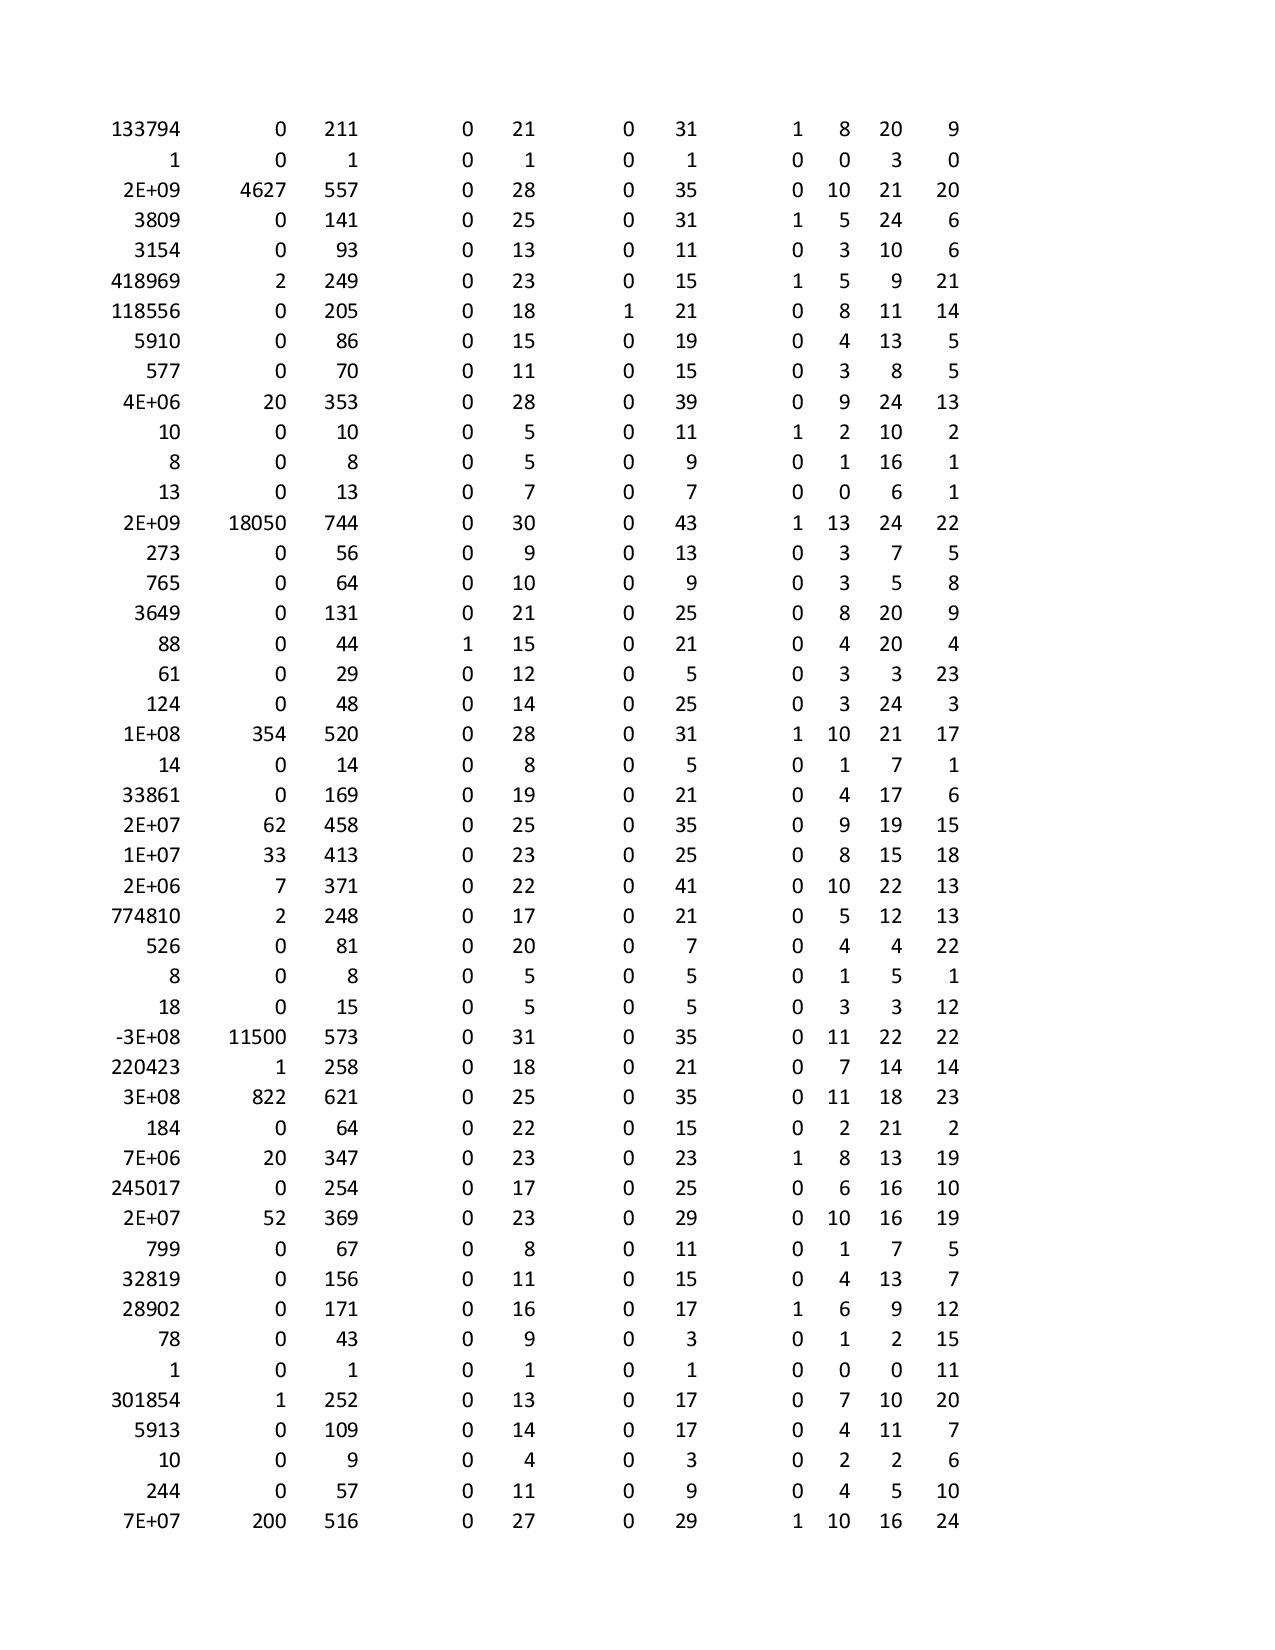
\includegraphics[width=2.5in]{51(2).jpg}
      \caption{Sample Profile Run2 in milliseconds.}
      \end{normalsize}
      \end{figure}
        
      \begin{figure}[htb]
      \begin{normalsize}  
      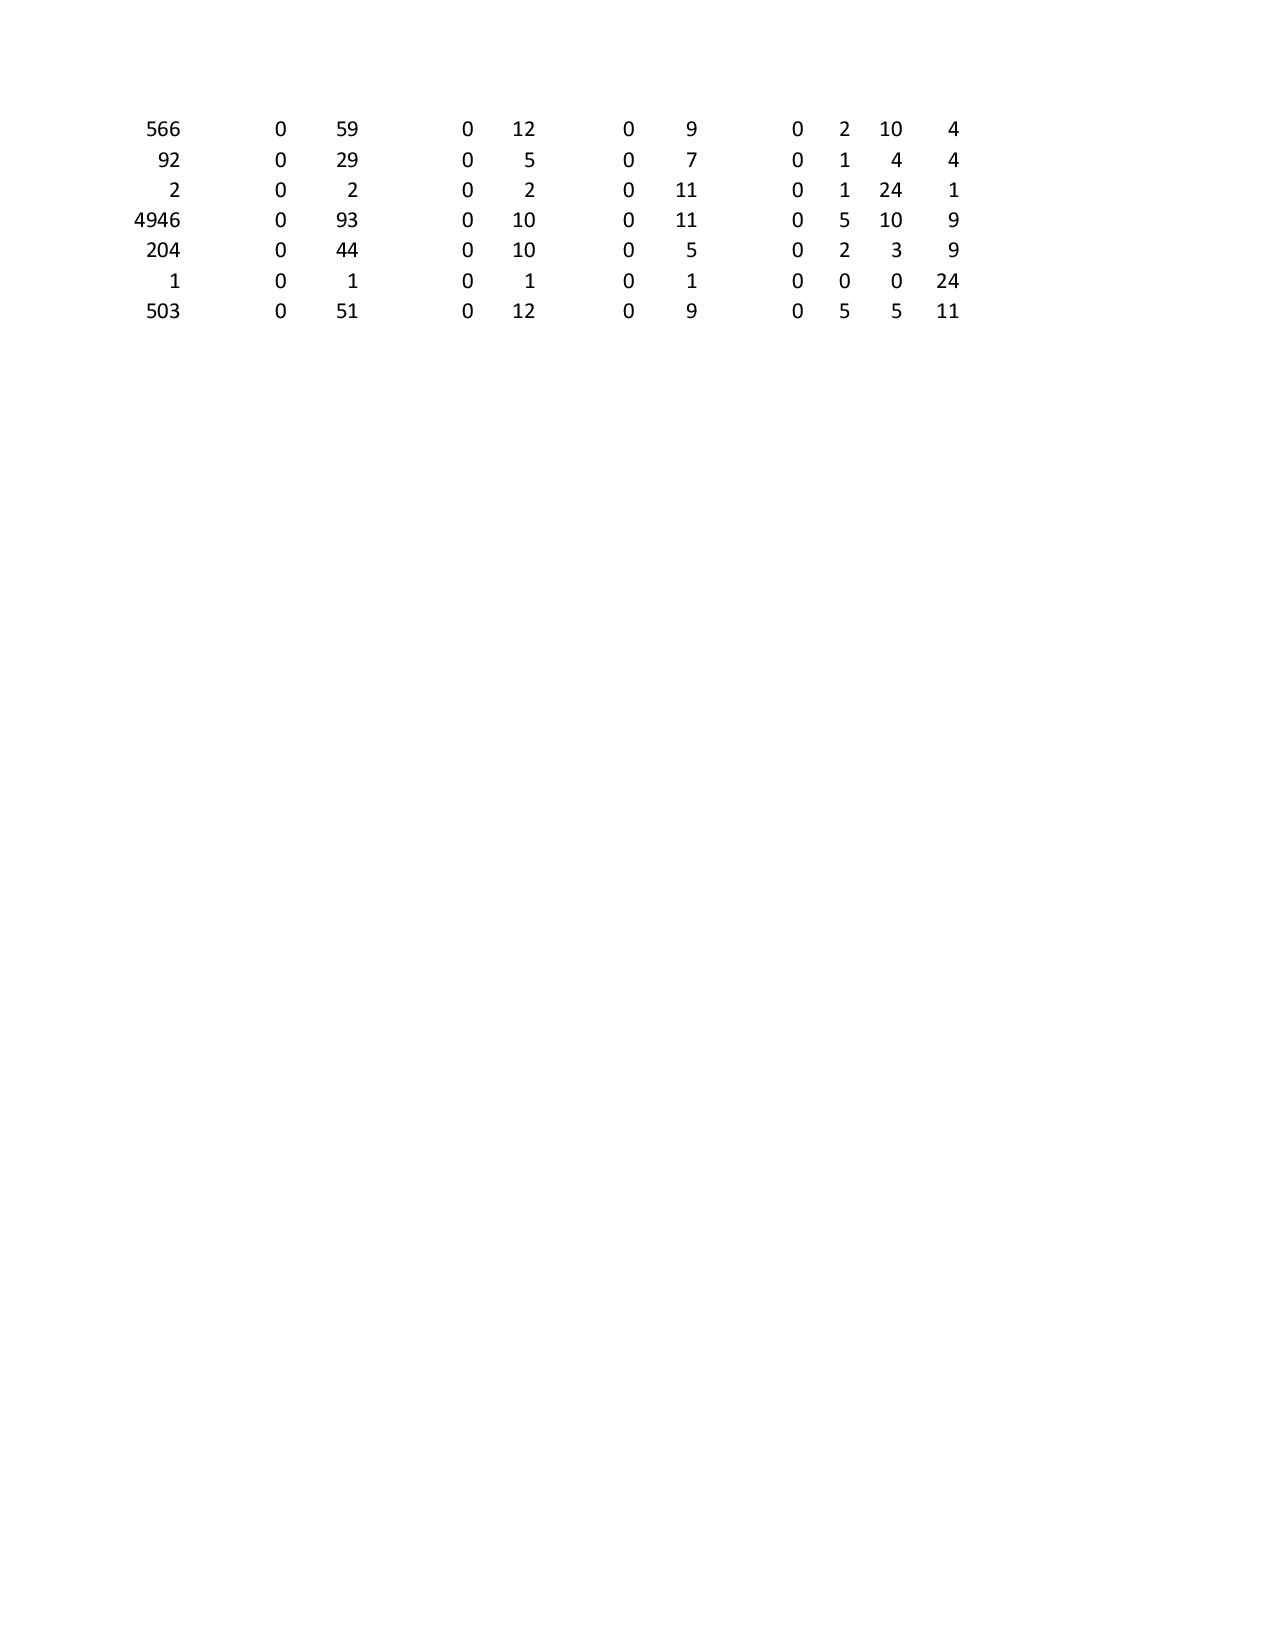
\includegraphics[width=2.5in]{51(3).jpg}
      \caption{Sample Profile Run3 in milliseconds.}
      
\end{normalsize}
\end{figure}
\clearpage
%}
%\end{enumerate}}
     

\section{Conclusion}
\label{current status}
This experimental project served to us as a great experience to learn more about the implementation of different algorithms such as Naïve Recursive, Meoization version, Dynamic programming, and Hirscberg. Each one of these algorithms implementation was based on the LCS computation, which was generated from two input strings. These inputs strings, in our case, were in two forms. First, we tested the algorithms with random whose length was varying randomly. Second, we tested the algorithms with strings of equal and different length, which were increasing linearly. Lastly, all tests were recorded by high level scripts in java, and analyzed by high level scripts in Matlab. Furthermore, we were able to learn how to utilize certain tools which were crucially important for the development of this report. These tools are Matlab and \LaTeX.
\newline

Matlab, we learned how to process and analyze data by classification. Using the necessary data for performance analysis, which includes the time efficiency and number of recursive calls. 
\newline

\LaTeX, we learned how to utilize this tool to professionally write our report. Also, we were able to learn how to manage image and formatting to technically write our documentation.
\newline 

In fact, the implementation of this project helped us to understand how to analyze the behavior of an algorithm. The factors that depend on the complexity of such algorithm. In brief, it taught us the importance of the performance of any algorithm. This means, the complexity of the algorithm matters as much as the memory usage for the development process. This would affect any system even if we have modern computer with advanced GPU.
\end{document}